\chapter{The Polar Front as a major biogeographic boundary in the Southern Ocean} 
\label{ch:polarfront}

Sections of this chapter have been previously published in \bibentry{Wilkins:2012td}.

\section{Summary}

\section{Introduction}


\section{Methods}
\subsection{Sampling and metagenomic sequencing}

Sampling\footnote{Sampling was performed by Jeffrey M. Hoffman and Jeffrey B. McQuaid} was conducted on board the RSV \emph{Aurora Australis} during cruise V3 \ac{CEAMARC/CASO} from 13 December 2007 -- 26 January 2008. 
This cruise occupied the SR3 latitudinal transect from Hobart, Australia (44\textdegree{} S) to the Mertz Glacier, Antarctica (67\textdegree{} S) within a longitudinal range of 140--150\textdegree{} E.
Nineteen samples (16 surface, 3 deep) were obtained along almost the entire latitudinal range \figref{fig:samplemap}.

% the sample map
\begin{figure}[!ht]
  \centering
  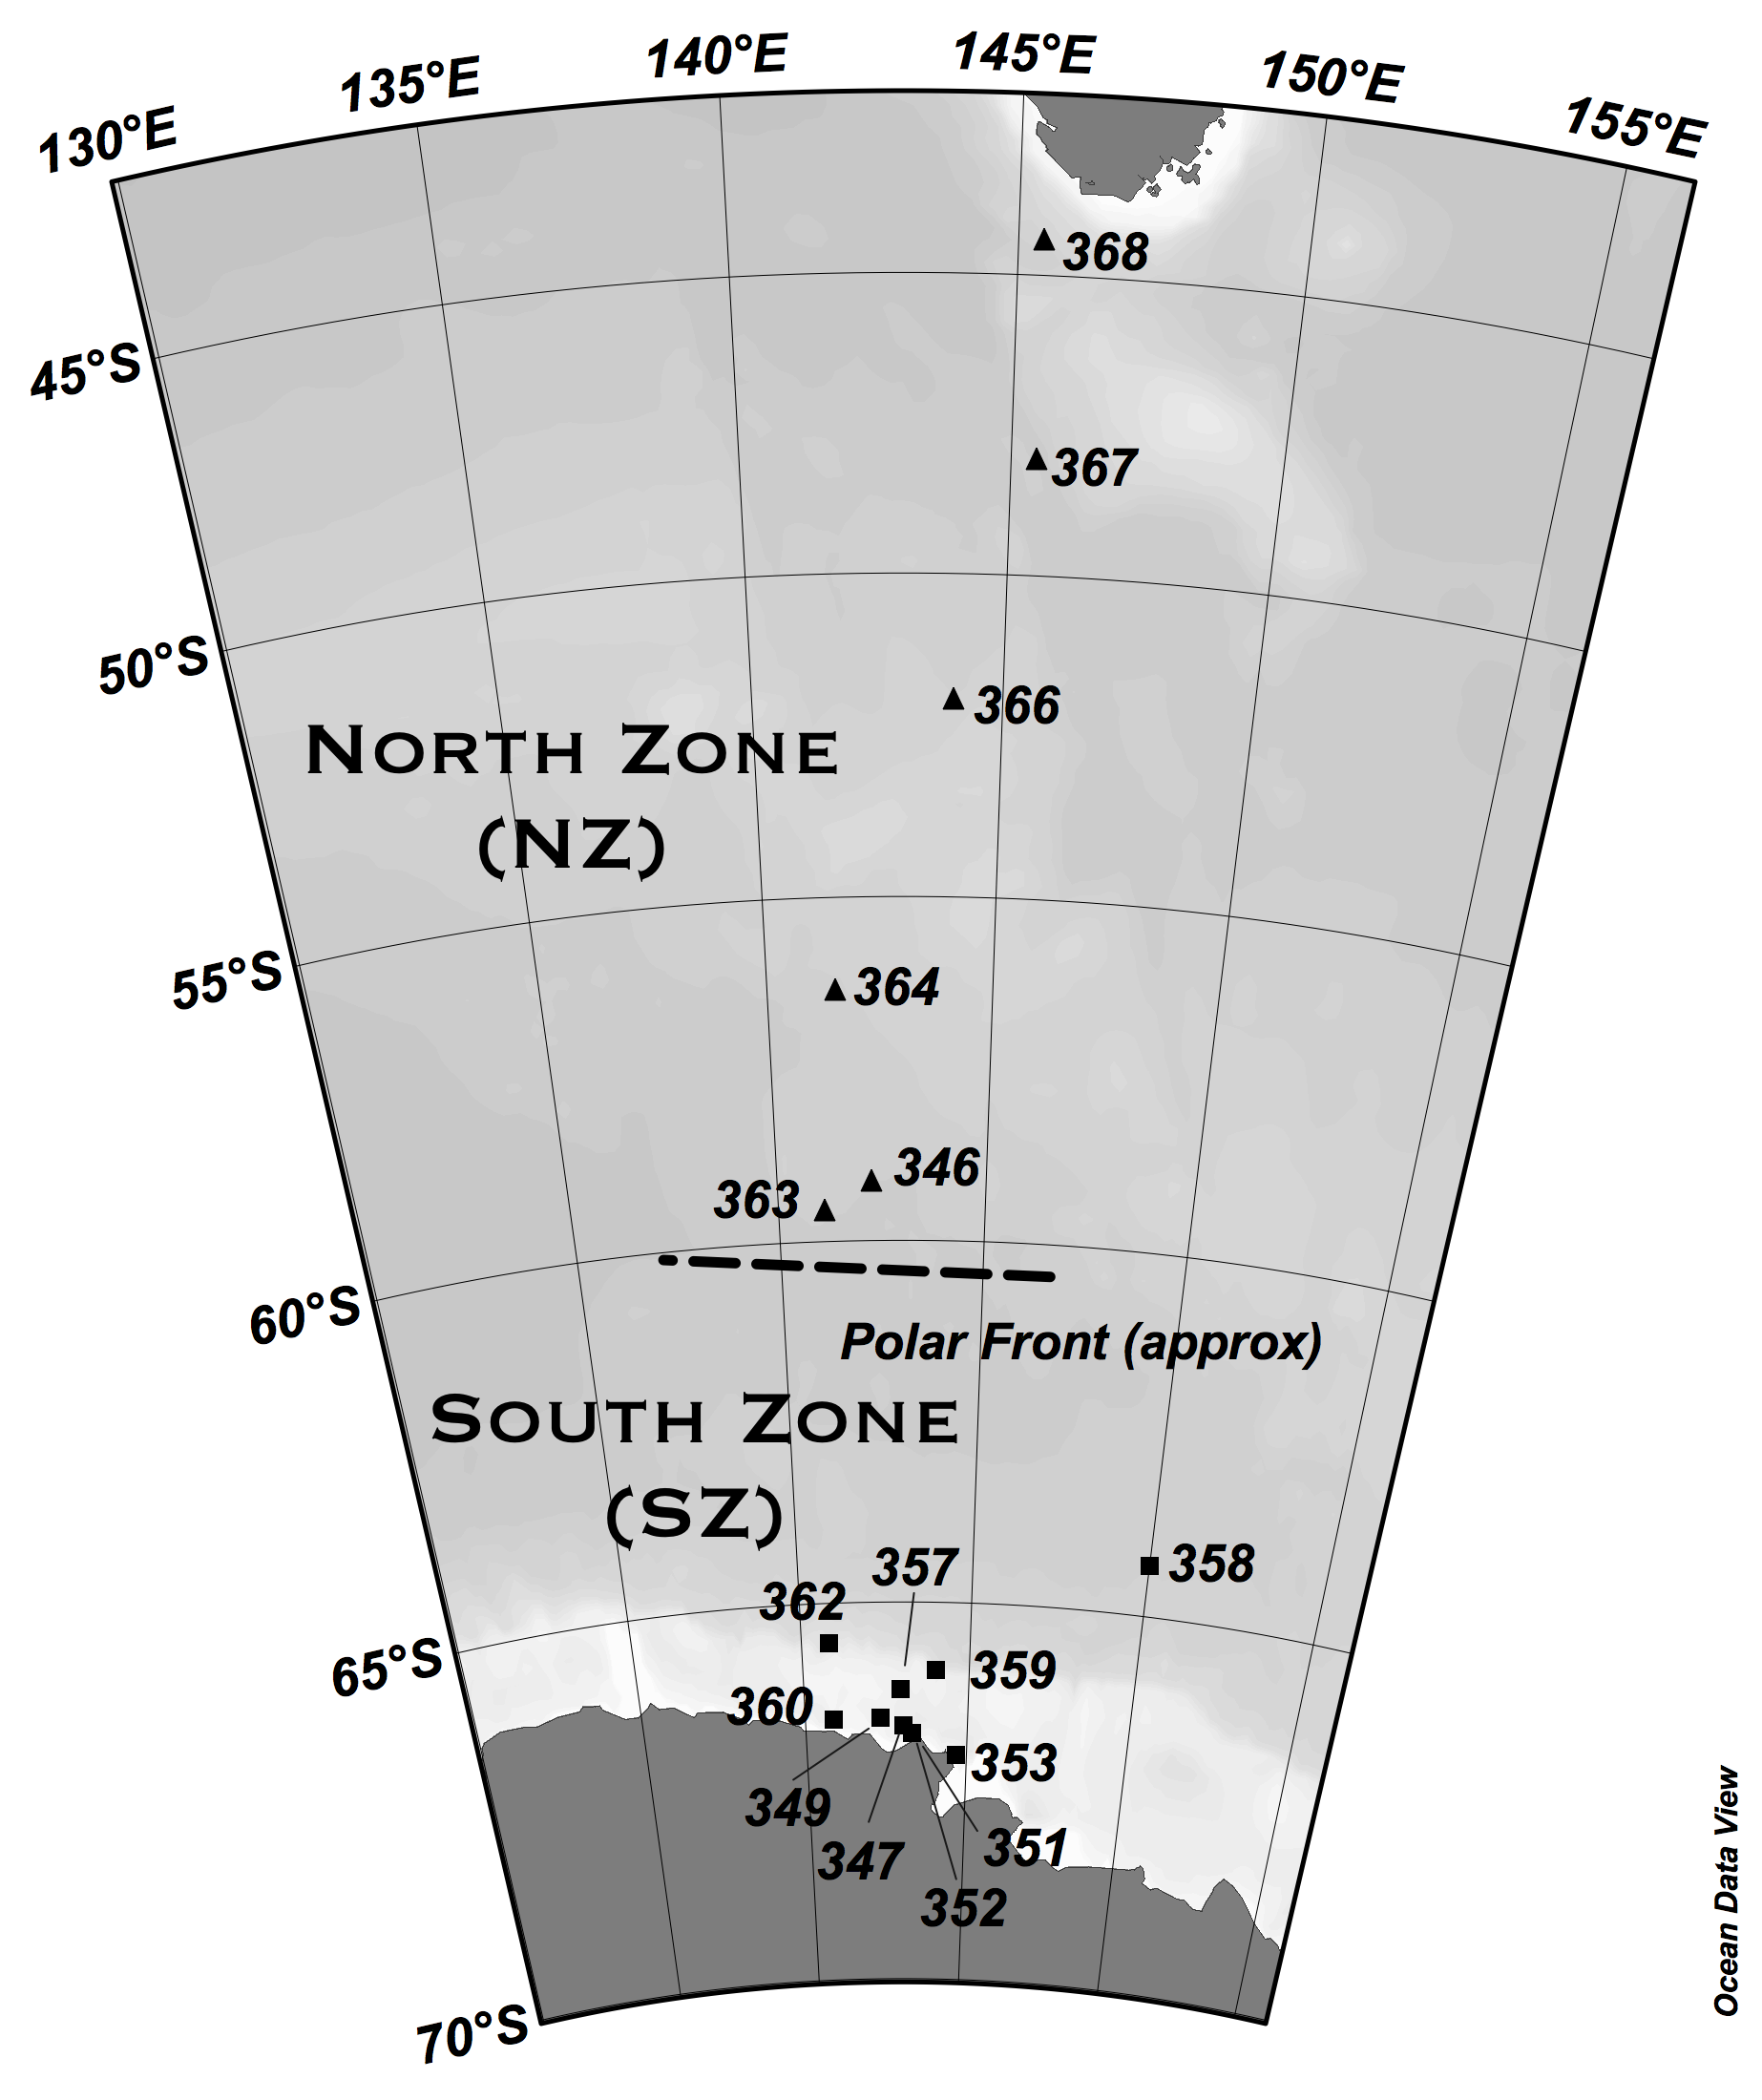
\includegraphics[width=\textwidth]{../polarfront/samplemap.png}
  \caption[Map showing sites of seawater samples used in the Polar Front study]{Sites of seawater samples used in this study. 
  Squares indicate surface samples from the North Zone; crosses samples from the South Zone. 
  The dashed line represents the Polar Front.}
  \label{fig:samplemap}
\end{figure}


A range of data were recorded by integrated instruments on the RSV \emph{Aurora Australis} including location, water column depth, water temperature, salinity, fluorescence and meterological data \tabref{tab:samplelist}.
These data were used to locate the \ac{PFZ} based on a surface temperature gradient of \textapprox{} 1.35 \textdegree{}C across a distance of 45--65 km, placing the \ac{PF} at approximately $-59.70$\textdegree{} of latitude, consistant with previous descriptions \cite{Moore:1999to,Sokolov:2002tc}.
Samples were accordingly grouped into ``North'' and ``South'' zones, while the three deep samples composed a ``Deep'' zone \tabref{tab:samplelist}.
The \ac{NZ} represents waters from the Subtropical, Subantarctic and \ac{PFZ} regions, while the \ac{SZ} represents the \ac{AZ}.

\begin{sidewaystable}
\sffamily
\caption[Details of samples used in Polar Front study]{\sffamily{}Sampling time, location and physicochemical properties of samples used in this study.
All data were retrieved from underway instruments aboard the RSV \textit{Aurora Australis}.}
\label{tab:samplelist}
\smallskip
\begin{tabularx}{\textheight}{lllXXXXXXXX}
\toprule
\textbf{Sample} & \textbf{Zone} & \textbf{Date} & \textbf{Latitude} & \textbf{Longitude} & \textbf{Water \linebreak Column \linebreak Depth (m)} & \textbf{Sample Depth (m)} & \textbf{Temperature (\textdegree{}C)} & \textbf{Salinity (PSU)} & \textbf{Fluorescence \linebreak (\textmu{}gL\textsuperscript{\textminus{}1})} & \textbf{Volume \linebreak filtered (L)}\\
\midrule

346 & North & 20/12/2007 & \textminus{}59.31 & 142.59 & 4294 & 2 & 2.9 & 33.75 & 0.3 & 500\\
347 & South & 23/12/2007 & \textminus{}66.02 & 142.74 & 450 & 2 & 0.6 & 34.20 & 4.0 & 250\\
349 & South & 27/12/2007 & \textminus{}66.57 & 142.32 & 370 & 1.5 & \textminus{}1.3 & 34.40 & 2.3 & 250\\
351 & South & 28/12/2007 & \textminus{}66.56 & 143.43 & 823 & 1.5 & \textminus{}0.6 & 34.30 & 1.3 & 500\\
352 & South & 29/12/2007 & \textminus{}66.77 & 143.32 & 164 & 2.5 & \textminus{}0.8 & 34.30 & 3.1 & 500\\
353 & South & 30/12/2007 & \textminus{}67.05 & 144.68 & 180 & 2 & \textminus{}1.8 & 34.40 & 0.3 & 500\\
357 & South & 05/01/2008 & \textminus{}66.17 & 143.02 & 580 & 2 & \textminus{}0.4 & 34.15 & 2.5 & 500\\
358 & South & 09/01/2008 & \textminus{}64.30 & 150.03 & 3550 & 2 & 0 & 33.55 & 0.5 & 500\\
359 & South & 12/01/2008 & \textminus{}66.19 & 143.53 & 540 & 2 & \textminus{}0.2 & 34.21 & 2.5 & 500\\
360 & South & 13/01/2008 & \textminus{}66.58 & 141.02 & 316 & 2 & \textminus{}0.7 & 34.04 & 6.2 & 500\\
362 & South & 19/01/2008 & \textminus{}65.54 & 140.83 & 1064 & 2 & 0.7 & 32.20 & 0.5 & 500\\
363 & North & 22/01/2008 & \textminus{}60.00 & 141.31 & 4473 & 2 & 3.3 & 33.77 & 0.1 & 500\\
364 & North & 23/01/2008 & \textminus{}56.70 & 141.88 & 3693 & 2 & 4 & 33.70 & 0.5 & 500\\
366 & North & 24/01/2008 & \textminus{}52.02 & 144.14 & 3180 & 2 & 7.6 & 33.84 & 0.3 & 500\\
367 & North & 25/01/2008 & \textminus{}48.25 & 145.90 & 3490 & 2 & 11 & 34.43 & 0.2 & 500\\
368 & North & 26/01/2008 & \textminus{}44.72 & 145.78 & 3201 & 2 & 14.8 & 34.96 & 1.3 & 560\\

\bottomrule
\end{tabularx}
\end{sidewaystable}


At each station, \textapprox{} 250--560 L of seawater was pumped from \textapprox{} 1.5--2.5 m below the sea surface into drums stored at ambient temperature on deck. 
In the case of deep samples, \textapprox{} 225--230 L of seawater was collected from Niskin bottles attached to a \ac{CTD} (SeaBird, Bellevue, USA).
Seawater samples were prefiltered through a 20 \micron{} plankton net, then filtrate was captured on sequential 3.0 \micron{} 0.8 \micron{} and 0.1 \micron{} 293 mm polyethersulfone membrane filters (Port Washington, USA), and immediately stored at $-20$ $^\circ$C \cite{Rusch:2007ez,Ng:2010cd}.

DNA extraction\footnote{DNA extraction was performed by Cynthia Andrews-Pfannkoch and others at the J. Craig Venter Institute} was performed at the J. Craig Venter Institute (Rockville, USA) as described in \citet{Rusch:2007ez}.
Pyrosequencing was performed on a GS20 FLX Titanium instrument (Roche, Branford, USA) also at the J. Craig Venter Institute as described in \citet{Lauro:2010jna}.
Duplicate reads and reads with many pyrosequencing errors were removed as described in \citet{Lauro:2010jna}.

\subsection{Phylogenetic analysis of metagenomic data}

\subsubsection{\softwarename{blast} comparison to RefSeq database}

A subset of the RefSeq microbial (bacterial and archaeal) genome database (release 41, retrieved May 31 2012 from \url{ftp://ftp.ncbi.nih.gov/refseq/release/}) was prepared by excluding sequences with the words ``shotgun'', ``contig'', ``partial'', ``end'' or ``part'' in their headers \cite{Angly:2009ip}.
Because this database was not expected to contain representative genomes for every species present, \acp{OTU} in this study are defined by the best species match to this database, and may for example represent congeners.

The metagenomic reads from each sample were compared against this database using \softwarename{tblastx}, with default parameters except for: E-value threshold $1.0\times{}10^{-3}$, cost to open gap 11, cost to extend gap 1, masking of query sequence by \softwarename{SEG} masking with lookup table only.
The outputs of all \softwarename{tblastx} searches against RefSeq were processed by \softwarename{minspec} (see section following), and hits not belonging to the minimal sets were removed.

\subsubsection{Identification of minimal species sets with \softwarename{minspec}}

A computational method to minimise false \ac{OTU} identifications and increase the accuracy of \ac{OTU} abundance estimates (\softwarename{minspec}) was developed and implemented in \softwarename{perl}\footnote{\softwarename{minspec} and the associated metagenomic simulation and validation scripts are open source and available at \url{https://github.com/wilkox/minspec}; a copy has also been provided in the supplementary information.}.
Following the approach of \citet{Ye:2009bl} to the parsimonious reconstruction of biochemical pathways (\softwarename{MinPath}), \softwarename{minspec} computes the smallest set of OTUs sufficient to explain a set of observed high-quality hits against RefSeq (or any other sequence database).
The minimal set computation is framed as a linear programming problem and solved with the \ac{GLPK} tool \ac{GLPSOL} (Free Software Foundation, Boston).
This approach eliminates many of the spurious \ac{OTU} identifications which result from reads with strong identity to more than one \ac{OTU}. 
The ``minimal species set'' is liable to exclude some low-abundance \acp{OTU}, but gives more faithful abundance estimates and eliminates many false positives.

To validate this approach and estimate error rates, simulated microbial assemblages were generated and simulated metagenomic sampling and \softwarename{blast} search was performed on each assemblage.
To simulate sequence identity between taxa, each simulated taxon went through up to fifty rounds in which another taxon was selected at random and deemed to have sequence identity with the first.
After each round, the this process was terminated with a 10\% probability to simulate an exponential curve of interrelatedness between taxa.
A random subset of the simulated taxa were then selected to form the simulated assemblage.
This allowed for the possibility of taxa in the assemblage having ``sequence identity'' to taxa outside it, thus representing the problem \softwarename{minspec} was designed to mitigate.
A simulated \softwarename{blast} search was then performed, in which a taxon was selected at random to generate a \softwarename{blast} hit.
To represent a lack of species evenness, taxa were more or less likely to produce a hit according to a logarithmic relationship with their rank within the assemblage, producing a naturalistic rank-abundance curve.
Each time a taxon was selected to produce a hit, other taxa with simulated sequence identidy were also selected to produce hits for that ``read'', again simulating the problem of a single read producing multiple hits to closely related taxa.

To fully explore the limits and reliability of \softwarename{minspec}, the simulated metagenomic experiment described above was performed with all possible permutations of the following parameters: number of simulated taxa [100, 1000, 10000, 50000, 100000]; size of simulated assemblage [1, 10, 100, 300, 500, 1000, 10000]; number of simulated metagenomic reads [10, 100, 1000, 10000, 100000, 200000, 500000].
Each permutation was repeated five times, except for those where the size of the assemblage would exceed the number of taxa simulated.
The resulting simulated \softwarename{blast} outputs were processed with \softwarename{minspec}, and the false positive (percentage of taxa not in the assemblage which nevertheless survived \softwarename{minspec} filtering) and false negative (percentage of taxa present in the assemblage which were not present after minspec filtering) rates calculated.
Because a high false negative rate can arise from undersampling, a problem in metagenomic studies both real and simulated, an additional ``false negative (\softwarename{minspec})'' metric was calculated, which excluded taxa which were present in the assemblage but through random chance did not generate any reads, the equivilant of ``unsampled rare taxa''.
This rate thus represented only false negatives attributable to \softwarename{minspec} itself.
Finally, as a measure of \softwarename{minspec}'s usefulness, the proportion of ``false'' taxa --- those which generated \softwarename{blast} hits but were not part of the assemblage --- that were succesfully removed by \softwarename{minspec} was calulated.

\subsubsection{\ac{OTU} abundances and variance between zones}

The relative \ac{OTU} abundances for each sample were determined using the \softwarename{perl} script \ac{GAAS} \cite{Angly:2009ip}.
Briefly, \ac{GAAS} estimates the relative abundance of \acp{OTU} from the number and quality of BLAST hits to each species, taking into account differences in genome size. 
\ac{GAAS} was run with the default settings. 
To normalise for reads which did not yield acceptable hits, the relative abundances for each sample were scaled by that sample's effective \softwarename{blast} hit rate. 
An \ac{OTU} profile was generated for each sample by encoding the scaled relative abundance of each \ac{OTU} from each size fraction as a separate variable.

To test the hypothesis that the oceanic zones harbour significantly different communities, \ac{ANOSIM} with 999 permutations was performed on a standardised, log-transformed Bray-Curtis resemblance matrix of \ac{OTU} profiles.
\ac{SIMPER} analysis was performed to identify the contribution of individual \acp{OTU} to differences between the zones. 
All statistical procedures were performed in \softwarename{PRIMER 6} as described by \citet{Clarke:2001ut}.

\subsection{Functional analysis of metagenomic data}

\subsubsection{\softwarename{blast} comparison to \ac{KEGG} database}

In order to identify functional differences between the zones, the set of metagenomic reads from each sample was compared against the \ac{KEGG} GENES database (retrieved July 2 2010 from \url{ftp://ftp.genome.jp/pub/kegg/genes/fasta/genes.pep}) with \softwarename{blastx}, with default parameters except for: maximum number of database sequence alignments 10; E-value threshold $1.0\times10^{-3}$; gap opening penalty 11; gap extension penalty 1; masking of query sequence by \softwarename{SEG} masking for lookup table only.

\subsubsection{Analysis of functional potential}

Genes identified by \softwarename{blastx} were aggregated to \ac{KEGG} ortholog groups according to the \ac{KEGG} Orthology schema (\url{ftp://ftp.genome.jp/pub/kegg/genes/ko}, retrieved Mar 29 2011), and ortholog group abundances calculated for each sample. 
Following \citet{Coleman:2010jj}, a read was considered a hit to a given ortholog group if the top three hits for that read (or all hits if fewer than three total hits) were to genes from the same ortholog group, and had bit scores \textgreater{} 40. 
If the bit score difference between any two top hits was greater than 30, only the hits above this difference were considered.

Ortholog group counts were then used to calculate the abundance of KEGG modules.
Because many ortholog groups are members of more than one module, the abundance $a_m$ of each module $m$ was calculated as 
\[
a_{m}=\sum_{K=1}^{n}\frac{C_{K}}{M_K}
\]
where $n$ is the number of ortholog groups $K$ belonging to module $m$, $C_{K}$ is the number of hits to ortholog group $K$, and $M_{K}$ is the total number of modules to which $K$ belongs.
To account for differences in sequencing depth between samples, module abundances were scaled to 500,000 reads per sample. 
To test the hypothesis that the \ac{NZ} and \ac{SZ} harbour significantly different functional potential, one-way \ac{ANOSIM} with 999 permutations was performed as above on a standardised, log-transformed Bray-Curtis distance resemblance matrix of the module and ortholog group profiles. 
A functional profile was generated for each sample by summing the scaled abundances of each module from all size fractions, and \ac{SIMPER} performed as above to identify modules which contributed highly to the variation in functional potential between the two zones. 
Modules with a high contribution to variance or otherwise of interest were then linked to taxonomy (``taxonomic decomposition'') by noting the genus of the organism associated with each gene in the \ac{KEGG} GENES database and thus calculating the relative contribution of each genus to each module's abundance. 
This allowed functional contributions to be putatively assigned to genera which were not identified in our taxonomic analysis, as the database included gene sequences for organisms for which a full genome was not available.

\section{Results}

\subsection{Metagenomic sequencing}
6.6 Gbp of 454 sequence data representing picoplankton in the size range 0.1 -- 3.0 \micron{} was obtained from 16 samples. 
After removal of low-quality reads, 454 sequencing yielded 157,507 -- 597,689 reads per sample (mean 354,399) of lengths ranging from 100 to 606 bp (mean 378).

\subsection{Phylogenetic analysis of metagenomic data}

The proportion of reads in each sample which yielded matches to RefSeq ranged from 25\% to 85\% (mean 62\%).
The most abundant \acp{OTU} in each sample are given in \tabreft{tab:topotus} and a full list of \ac{OTU} abundances in the supplementary material \suppfile{PF-all-OTUs.csv}.
All samples and size fractions exhibited very low \ac{OTU} evenness \figref{fig:rankabundance}.

\begin{sidewaystable}
\sffamily
\caption[Twenty most abundant \acp{OTU}]{\sffamily{}Relative abundances (as percentages) of the twenty most abundant \acp{OTU} identified in this study, in each zone and size fraction.}
\label{tab:topotus}
\smallskip
\begin{tabularx}{\textheight}{Xlllllllll}
\toprule
OTU & \multicolumn{3}{c}{North} & \multicolumn{3}{c}{South} & \multicolumn{3}{c}{Deep}\\
\cmidrule(r){2-4}
\cmidrule(r){5-7}
\cmidrule(r){8-10}
& 0.1 \micron & 0.8 \micron & 3.0 \micron & 0.1 \micron & 0.8 \micron & 3.0 \micron & 0.1 \micron & 0.8 \micron & 3.0 \micron\\
\midrule

\candidatusfull{Pelagibacter ubique} HTCC1062 & 61.76 & 25.00 & 23.87 & 58.85 & 22.40 & 17.61 & 37.05 & 24.56 & 17.66\\
\speciesfull{Nitrosopumilus maritimus} SCM1 & 0.01996 & 0.01438 & 0.009508 & 1.076 & 1.309 & 1.210 & 19.09 & 9.463 & 17.77\\
\candidatusfull{Ruthia magnifica} str. Cm (\speciesfull{Calyptogena magnifica}) & 0.6699 & 0.6458 & 0.5484 & 2.987 & 2.616 & 1.025 & 3.945 & 4.601 & 2.264\\
\genus{Roseobacter} sp. OCh114 & 0.3125 & 2.932 & 1.588 & 0.4477 & 3.994 & 2.657 & 0.1259 & 1.228 & 0.6792\\
\genus{Synechococcus} sp. CC9902 & 0.1081 & 9.837 & 4.973 & 0.0007484 & 0.004156 & 0.09733 & 0.002846 & 0.01502 & 0.01058\\
\speciesfull{Silicibacter pomeroyi} DSS-3 & 0.2578 & 2.286 & 1.154 & 0.3070 & 2.505 & 1.576 & 0.1224 & 0.9417 & 0.4988\\
\speciesfull{Gramella forsetii} strain KT0803 & 0.2412 & 1.210 & 1.755 & 0.4993 & 2.347 & 1.890 & 0.2078 & 0.6179 & 0.5173\\
\candidatusfull{Vesicomyosocius okutanii} strain HA & 0.4634 & 0.4642 & 0.2078 & 1.970 & 1.807 & 0.2174 & 2.480 & 2.662 & 1.167\\
\speciesfull{Robiginitalea biformata} strain HTCC2501 & 0.2751 & 1.099 & 1.297 & 0.4722 & 1.878 & 1.405 & 0.2265 & 0.6188 & 0.6946\\
\speciesfull{Flavobacterium psychrophilum} strain JIP02/86 & 0.1718 & 0.8409 & 1.224 & 0.4316 & 1.960 & 1.598 & 0.1599 & 0.4744 & 0.6001\\
\genus{Synechococcus} sp. CC9311 & 0.03014 & 4.624 & 4.409 & 0.0007221 & 0.002778 & 0.02764 & 0.001580 & 0.002863 & 0.009241\\
\candidatusfull{Puniceispirillum marinum} IMCC1322 & 0.6444 & 2.077 & 1.267 & 0.3586 & 1.377 & 0.7109 & 0.3425 & 1.062 & 0.5345\\
\genus{Silicibacter} sp. TM1040 & 0.2274 & 1.652 & 0.8738 & 0.2709 & 1.803 & 1.233 & 0.07665 & 0.5890 & 0.2957\\
\genus{Jannaschia} sp. DFL-12 & 0.1776 & 1.378 & 0.7350 & 0.2443 & 1.692 & 0.8009 & 0.07338 & 0.6515 & 0.3078\\
\speciesfull{Zunongwangia profunda} strain SM-A87 & 0.1522 & 0.7487 & 1.059 & 0.2968 & 1.410 & 1.204 & 0.1353 & 0.3478 & 0.4971\\
\genus{Colwellia} sp. 34H & 0.02345 & 0.3636 & 2.736 & 0.05207 & 0.5140 & 1.041 & 0.05137 & 0.4687 & 0.8013\\
\speciesfull{Coraliomargarita akajimensis} strain DSM 45221 & 0.03698 & 0.07573 & 0.1197 & 0.1154 & 1.543 & 1.680 & 0.02614 & 0.3040 & 0.2740\\
\genus{Jannaschia} sp. CCS1 & 0.1173 & 0.9344 & 0.4784 & 0.1711 & 1.230 & 0.8239 & 0.05865 & 0.4462 & 0.2118\\
\speciesfull{Pseudoalteromonas atlantica} strain T6c & 0.01251 & 0.4772 & 1.993 & 0.02270 & 0.4089 & 1.132 & 0.02634 & 0.2143 & 0.7459\\
\speciesfull{Saccharophagus degradans} strain 2-40 & 0.06532 & 0.4325 & 0.5429 & 0.1289 & 1.072 & 0.8663 & 0.07798 & 0.2844 & 0.3165\\
\speciesfull{Flavobacterium johnsoniae} strain UW101 & 0.08822 & 0.4220 & 0.6141 & 0.2034 & 0.9389 & 0.8578 & 0.07545 & 0.2255 & 0.3300\\
\speciesfull{Capnocytophaga ochracea} strain DSM 7271 & 0.1143 & 0.4830 & 0.5399 & 0.2314 & 0.8815 & 0.6814 & 0.08964 & 0.2840 & 0.5043\\
\genus{Marinomonas} sp. MWYL1 & 0.03777 & 0.2529 & 0.3026 & 0.1514 & 1.300 & 0.7006 & 0.07393 & 0.2439 & 0.2155\\
\speciesfull{Cellvibrio japonicus} strain Ueda107 & 0.05884 & 0.3080 & 0.3231 & 0.1155 & 0.9917 & 0.4713 & 0.06774 & 0.2981 & 0.2549\\
\speciesfull{Marinobacter hydrocarbonoclasticus} VT8 & 0.04093 & 0.2889 & 0.3883 & 0.08418 & 0.7195 & 0.3848 & 0.1250 & 0.6667 & 1.066\\
\speciesfull{Pseudoalteromonas haloplanktis} strain TAC125 & 0.01389 & 0.2505 & 0.8896 & 0.03427 & 0.3561 & 0.6530 & 0.1092 & 1.203 & 0.1503\\
\speciesfull{Teredinibacter turnerae} strain T7901 & 0.05665 & 0.3051 & 0.3081 & 0.1138 & 0.9174 & 0.5127 & 0.06558 & 0.2649 & 0.1885\\
\speciesfull{Acinetobacter baumannii} strain SDF & 0.004886 & 0.007187 & 0.4073 & 0.006260 & 0.04218 & 1.459 & 0.004285 & 0.01229 & 0.3155\\

\bottomrule
\end{tabularx}
\end{sidewaystable}

% the sample map
\begin{figure}
  \centering
  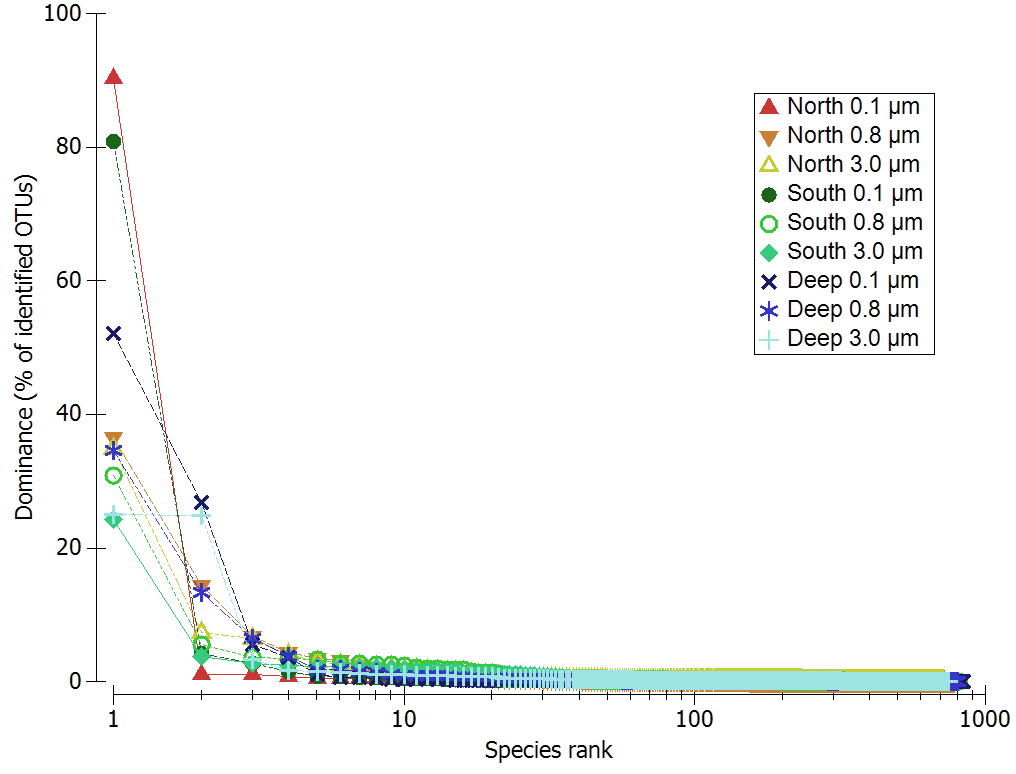
\includegraphics[width=\textwidth]{../polarfront/rankabundance.png}
  \caption[Rank-abundance curves for OTUs in each zone and size fraction]{Rank-abundance curves for OTUs identified in each zone and size fraction. The dominance of a given OTU is its relative abundance as a percentage of all identified OTUs. The x-axis is scaled logarithmically. Generated using \softwarename{PRIMER 6}.}
  \label{fig:rankabundance}
\end{figure}


\ac{ANOSIM} analysis showed that the zones harbor significantly different microbial communities (R = 0.451, p < 0.004). 
\ac{SIMPER} was performed in order to identify the contribution of individual \acp{OTU} to the difference between the \ac{NZ} and \ac{SZ}. 
The results for the highest contributors are provided in \tabreft{tab:otussimper}, and are graphically summarised for all \acp{OTU} in \figreft{fig:taxotreemap}.

\begin{sidewaystable}
\sffamily
\begin{center}
\caption[Highest-contributing \acp{OTU} to the difference between the North and South zones]{\sffamily{}
The thirty \acp{OTU} with the highest contributions to the difference between the \ac{NZ} and \ac{SZ}. 
  Abundances are zonal averages and have been standardised and log-transformed.
  As each \ac{OTU} on each size fraction was encoded as a separate variable in the \ac{SIMPER} analysis, the size fraction is given after each \ac{OTU} name.
  }
\label{tab:otussimper}
\begin{tabular}{llll}
\toprule
\textbf{OTU} & \textbf{Abundance} & \textbf{Abundance} & \textbf{Contribution to}\\
& \textbf{South} & \textbf{North} & \textbf{variance (\%)}\\

\midrule
\genus{Synechococcus} sp. CC9311 0.8 \micron & 0.00 & 1.08 & 2.88\\
\genus{Synechococcus} sp. CC9902 0.8 \micron & 0.00 & 1.04 & 2.81\\
\genus{Synechococcus} sp. CC9311 3.0 \micron & 0.01 & 0.98 & 2.59\\
\genus{Synechococcus} sp. CC9902 3.0 \micron & 0.04 & 0.76 & 2.03\\
\candidatusfull{Pelagibacter ubique} HTCC1062 3.0 \micron & 1.97 & 2.40 & 1.97\\
\candidatusfull{Ruthia magnifica} str. Cm (\speciesfull{Calyptogena magnifica}) 0.1 \micron & 0.82 & 0.25 & 1.57\\
\genus{Colwellia} sp. 34H 3.0 \micron & 0.34 & 0.66 & 1.32\\
\candidatusfull{Ruthia magnifica} str. Cm (\speciesfull{Calyptogena magnifica}) 0.8 \micron & 0.74 & 0.25 & 1.32\\
\candidatusfull{Pelagibacter ubique} HTCC1062 0.8 \micron & 2.32 & 2.48 & 1.32\\
\candidatusfull{Vesicomyosocius okutanii} strain HA 0.1 \micron & 0.62 & 0.18 & 1.20\\
\speciesfull{Coraliomargarita akajimensis} strain DSM 45221 0.8 \micron & 0.48 & 0.04 & 1.13\\
\speciesfull{Coraliomargarita akajimensis} strain DSM 45221 3.0 \micron & 0.49 & 0.06 & 1.10\\
\genus{Roseobacter} sp. OCh 114 0.8 \micron & 1.01 & 0.81 & 1.08\\
\speciesfull{Pseudoalteromonas atlantica} strain T6c 3.0 \micron & 0.38 & 0.54 & 1.08\\
\candidatusfull{Vesicomyosocius okutanii} strain HA 0.8 \micron & 0.57 & 0.19 & 1.04\\
\speciesfull{Acinetobacter baumannii} strain SDF 3.0 \micron & 0.45 & 0.18 & 0.95\\
\speciesfull{Gramella forsetii} strain KT0803 0.8 \micron & 0.72 & 0.43 & 0.94\\
\genus{Marinomonas} sp. MWYL1 0.8 \micron & 0.46 & 0.11 & 0.92\\
\genus{Roseobacter} sp. OCh 114 3.0 \micron & 0.76 & 0.54 & 0.91\\
\speciesfull{Flavobacterium psychrophilum} strain JIP02/86 0.8 \micron & 0.63 & 0.32 & 0.89\\
\speciesfull{Silicibacter pomeroyi} DSS-3 0.8 \micron & 0.75 & 0.69 & 0.86\\
\speciesfull{Brachyspira hyodysenteriae} strain WA1 3.0 \micron & 0.47 & 0.19 & 0.84\\
\candidatusfull{Ruthia magnifica} str. Cm (\speciesfull{Calyptogena magnifica}) 3.0 \micron & 0.34 & 0.21 & 0.82\\
\speciesfull{Pseudoalteromonas haloplanktis} strain TAC125 3.0 \micron & 0.22 & 0.33 & 0.77\\
\speciesfull{Robiginitalea biformata} strain HTCC2501 0.8 \micron & 0.61 & 0.40 & 0.74\\
\speciesfull{Nitrosopumilus maritimus} SCM1 0.1 \micron & 0.27 & 0.01 & 0.72\\
\speciesfull{Gramella forsetii} strain KT0803 3.0 \micron & 0.59 & 0.59 & 0.71\\
\speciesfull{Lysinibacillus sphaericus} strain C3-41 3.0 \micron & 0.29 & 0.02 & 0.71\\
\speciesfull{Nitrosopumilus maritimus} SCM1 0.8 \micron & 0.25 & 0.01 & 0.70\\
\speciesfull{Silicibacter} sp. TM1040 0.8 \micron & 0.59 & 0.55 & 0.69\\

\bottomrule
\end{tabular}
\end{center}
\end{sidewaystable}

\begin{figure}[!ht]
  \centering
  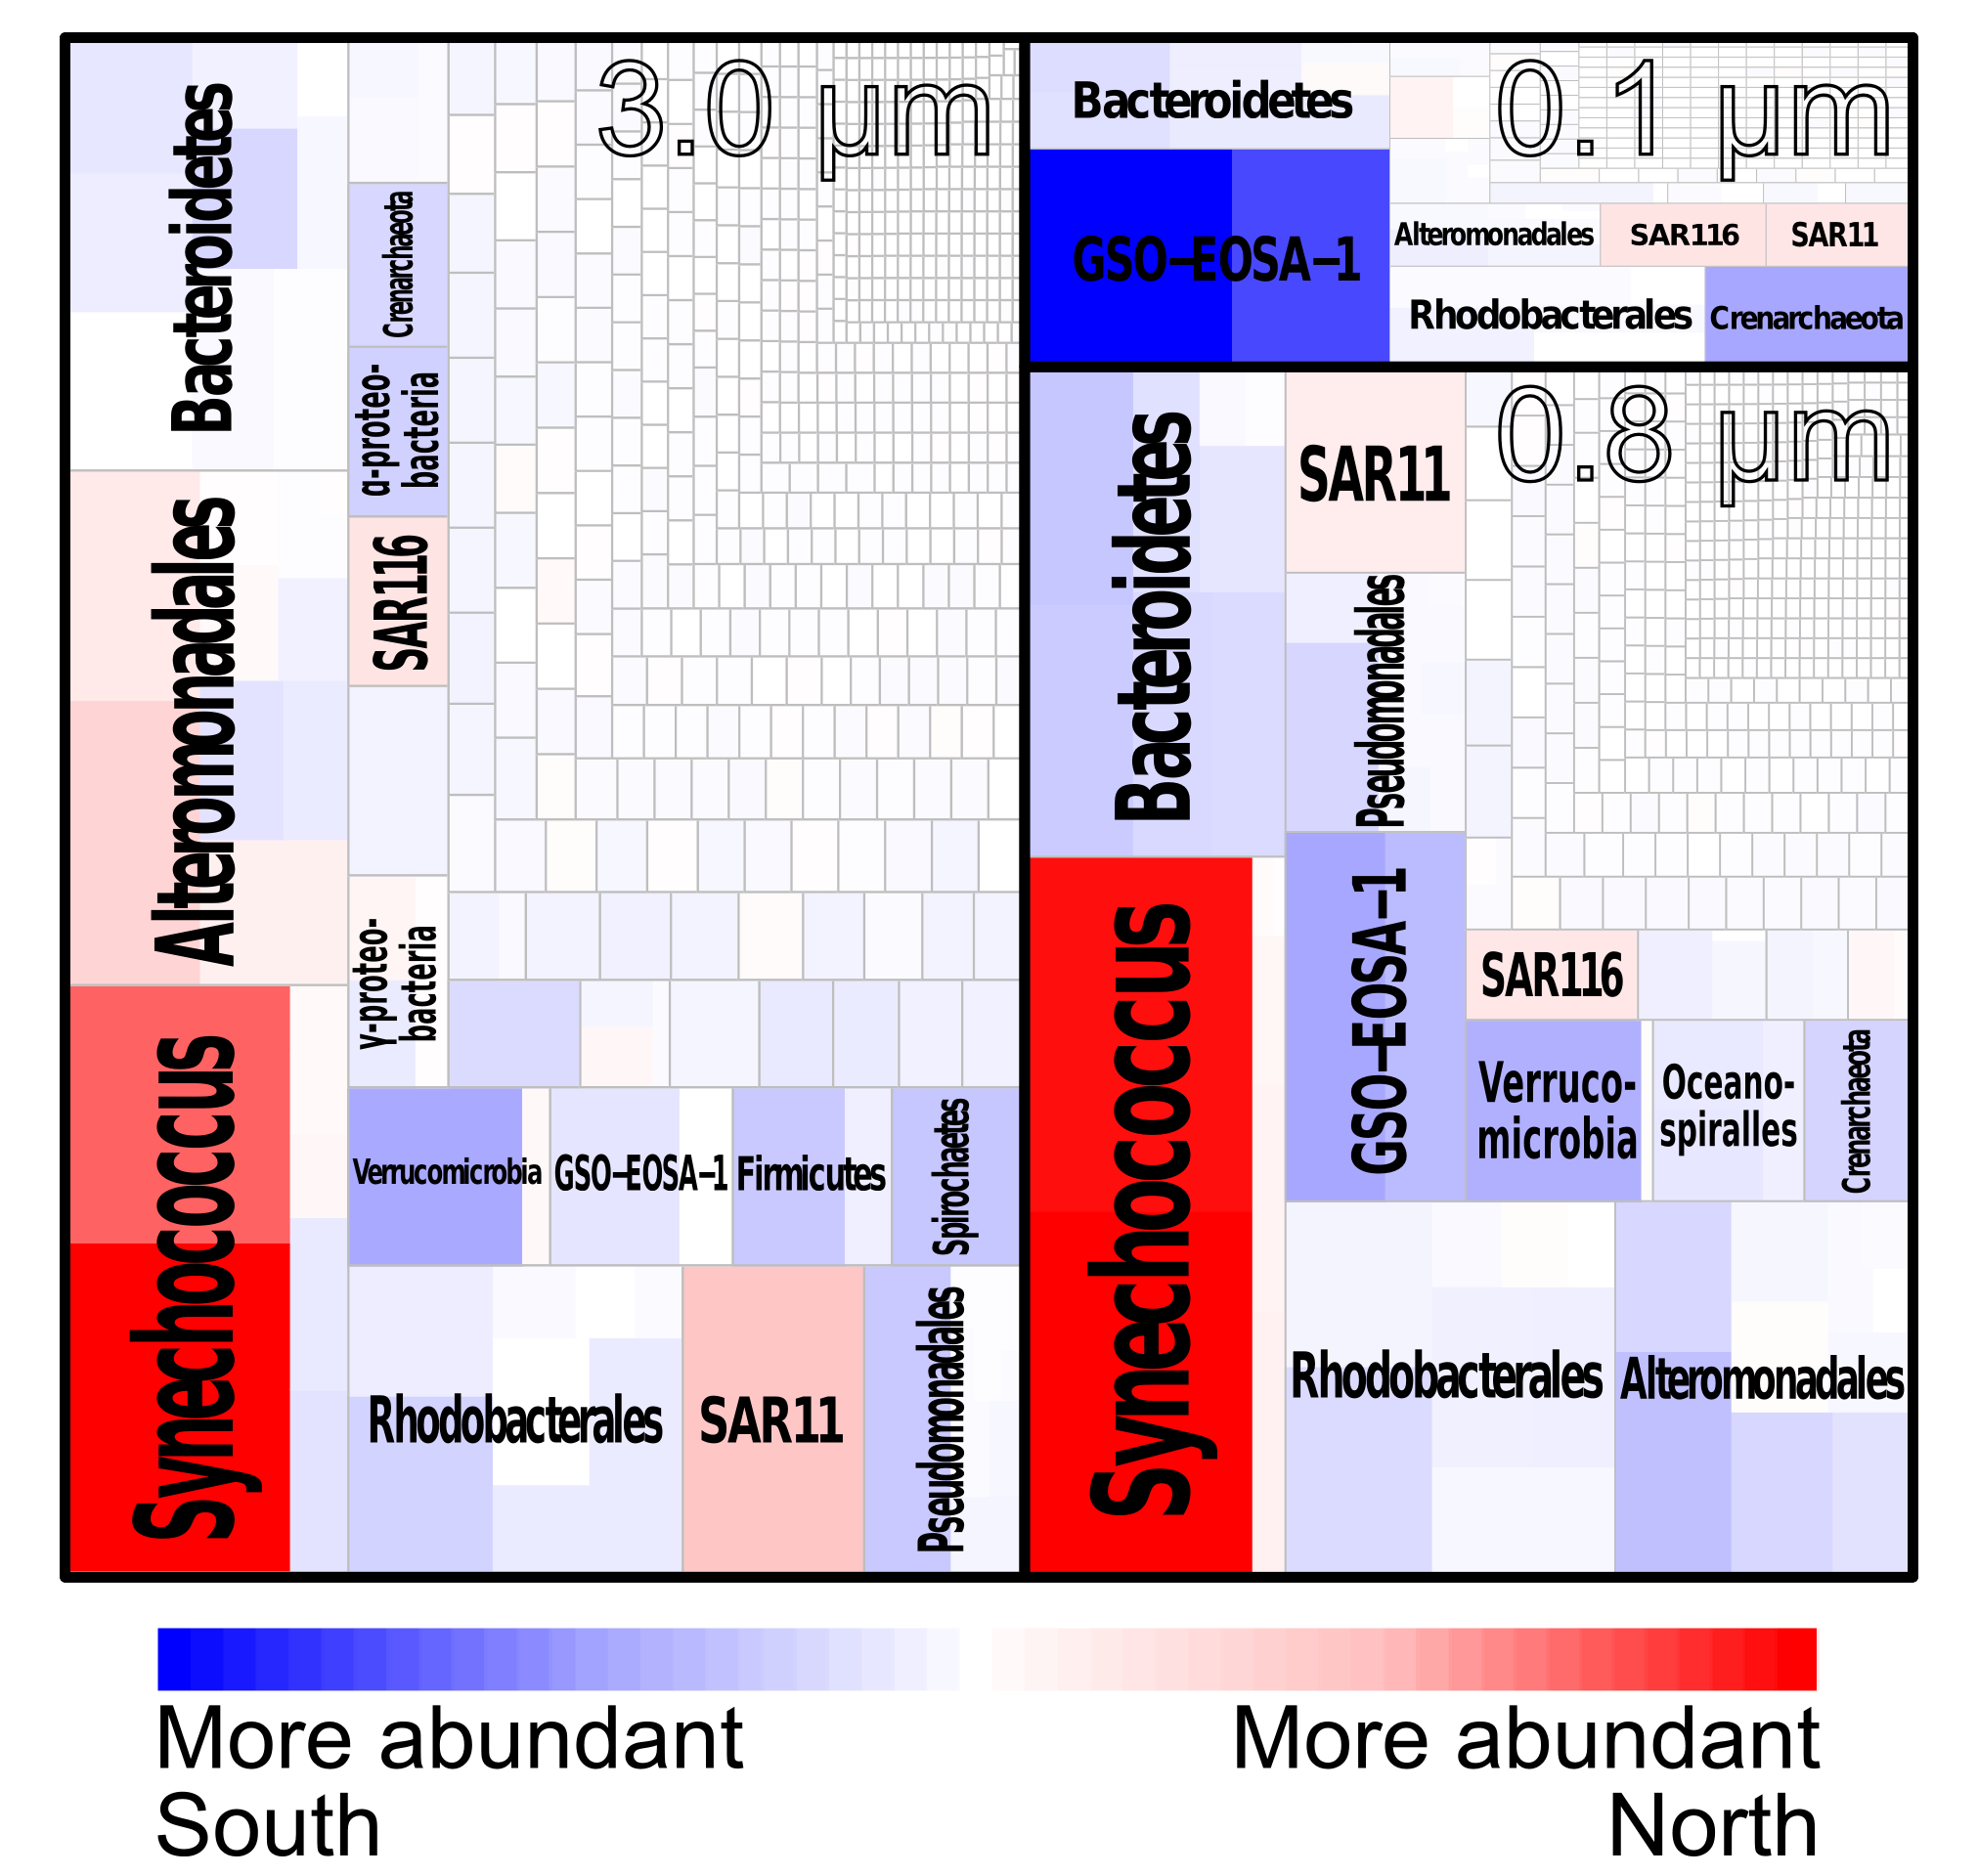
\includegraphics[width=\textwidth]{../polarfront/taxotreemap.png}
  \caption[Contribution of \acp{OTU} to variance between the North and South zones]{Contribution of \acp{OTU} to variance between the North and South zones, and differential abundance of \acp{OTU} from each size fraction between the two zones.
Each coloured (red or blue) rectangle represents an OTU identified through analysis of BLAST matches between SO metagenome data and the RefSeq database.
The area of each rectangle as a proportion of the total plot area corresponds to that \ac{OTU}'s contribution to the total variance between the two zones.
The colour of each rectangle corresponds to difference in relative abundance of that OTU between the zones, with blue indicating a higher relative abundance south of the PF, and red a higher abundance north of the PF.
\acp{OTU} from clades or taxonomic ranks of interest have been grouped, with labels in bold and groups separated by gray lines. 
Groups and \acp{OTU} with a low contribution to variance which were not grouped are unlabeled.
\acp{OTU} from each size fraction have also been grouped, with labels in black outline and size fractions separated by thick black lines. 
The data used to generate this figure are given in the supplementary material \suppfile{PF-OTUs-SIMPER.csv}.
  }
  \label{fig:taxotreemap}
\end{figure}


The \ac{SIMPER} analysis found that no single \ac{OTU} contributed more than 2.9\% of variance and 74\% of variance was contributed by \acp{OTU} with a contribution less than 1\%. 
There was also a large difference in the contribution to variance of the three size fractions, with approximately 52\% of all variance contributed by \acp{OTU} from the 3.0 \micron{} fraction, 37\% by the 0.8 \micron{} fraction, and 9\% by the 0.1 \micron{} fraction.
Notably, \acp{OTU} within several taxonomic groups that had high contribution to variance covaried in their relative representation in the \ac{NZ} and \ac{SZ}.
For example, Bacteroidetes and GSO-EOSA-1 representatives were on average more abundant in the \ac{SZ}; while \emph{Prochlorococcus} and \emph{Synechococcus} spp., SAR11 and SAR116 were on average more abundant in the \ac{NZ} \figref{fig:taxotreemap}.
Some groups, such as the Alteromonadales, had variable relative representation depending on size fraction.

\subsubsection{Validation of \softwarename{minspec}}
TODO maybe this needs to be broken out into a seperate small chapter?
TODO at the very least this belongs in Discussion.

Repeated simulated metagenomic experiments with a wide range of permutations of parameters indicated that \softwarename{minspec} was reliable and able to substantially reduce the rate of false positive \ac{OTU} identifications, although its effectiveness varied with the parameters of the assemblage and metagenomic experiment.

\begin{figure}
\centering

\begin{tabular}{cc}

\begin{subfigure}[b]{0.5\textwidth}
\centering
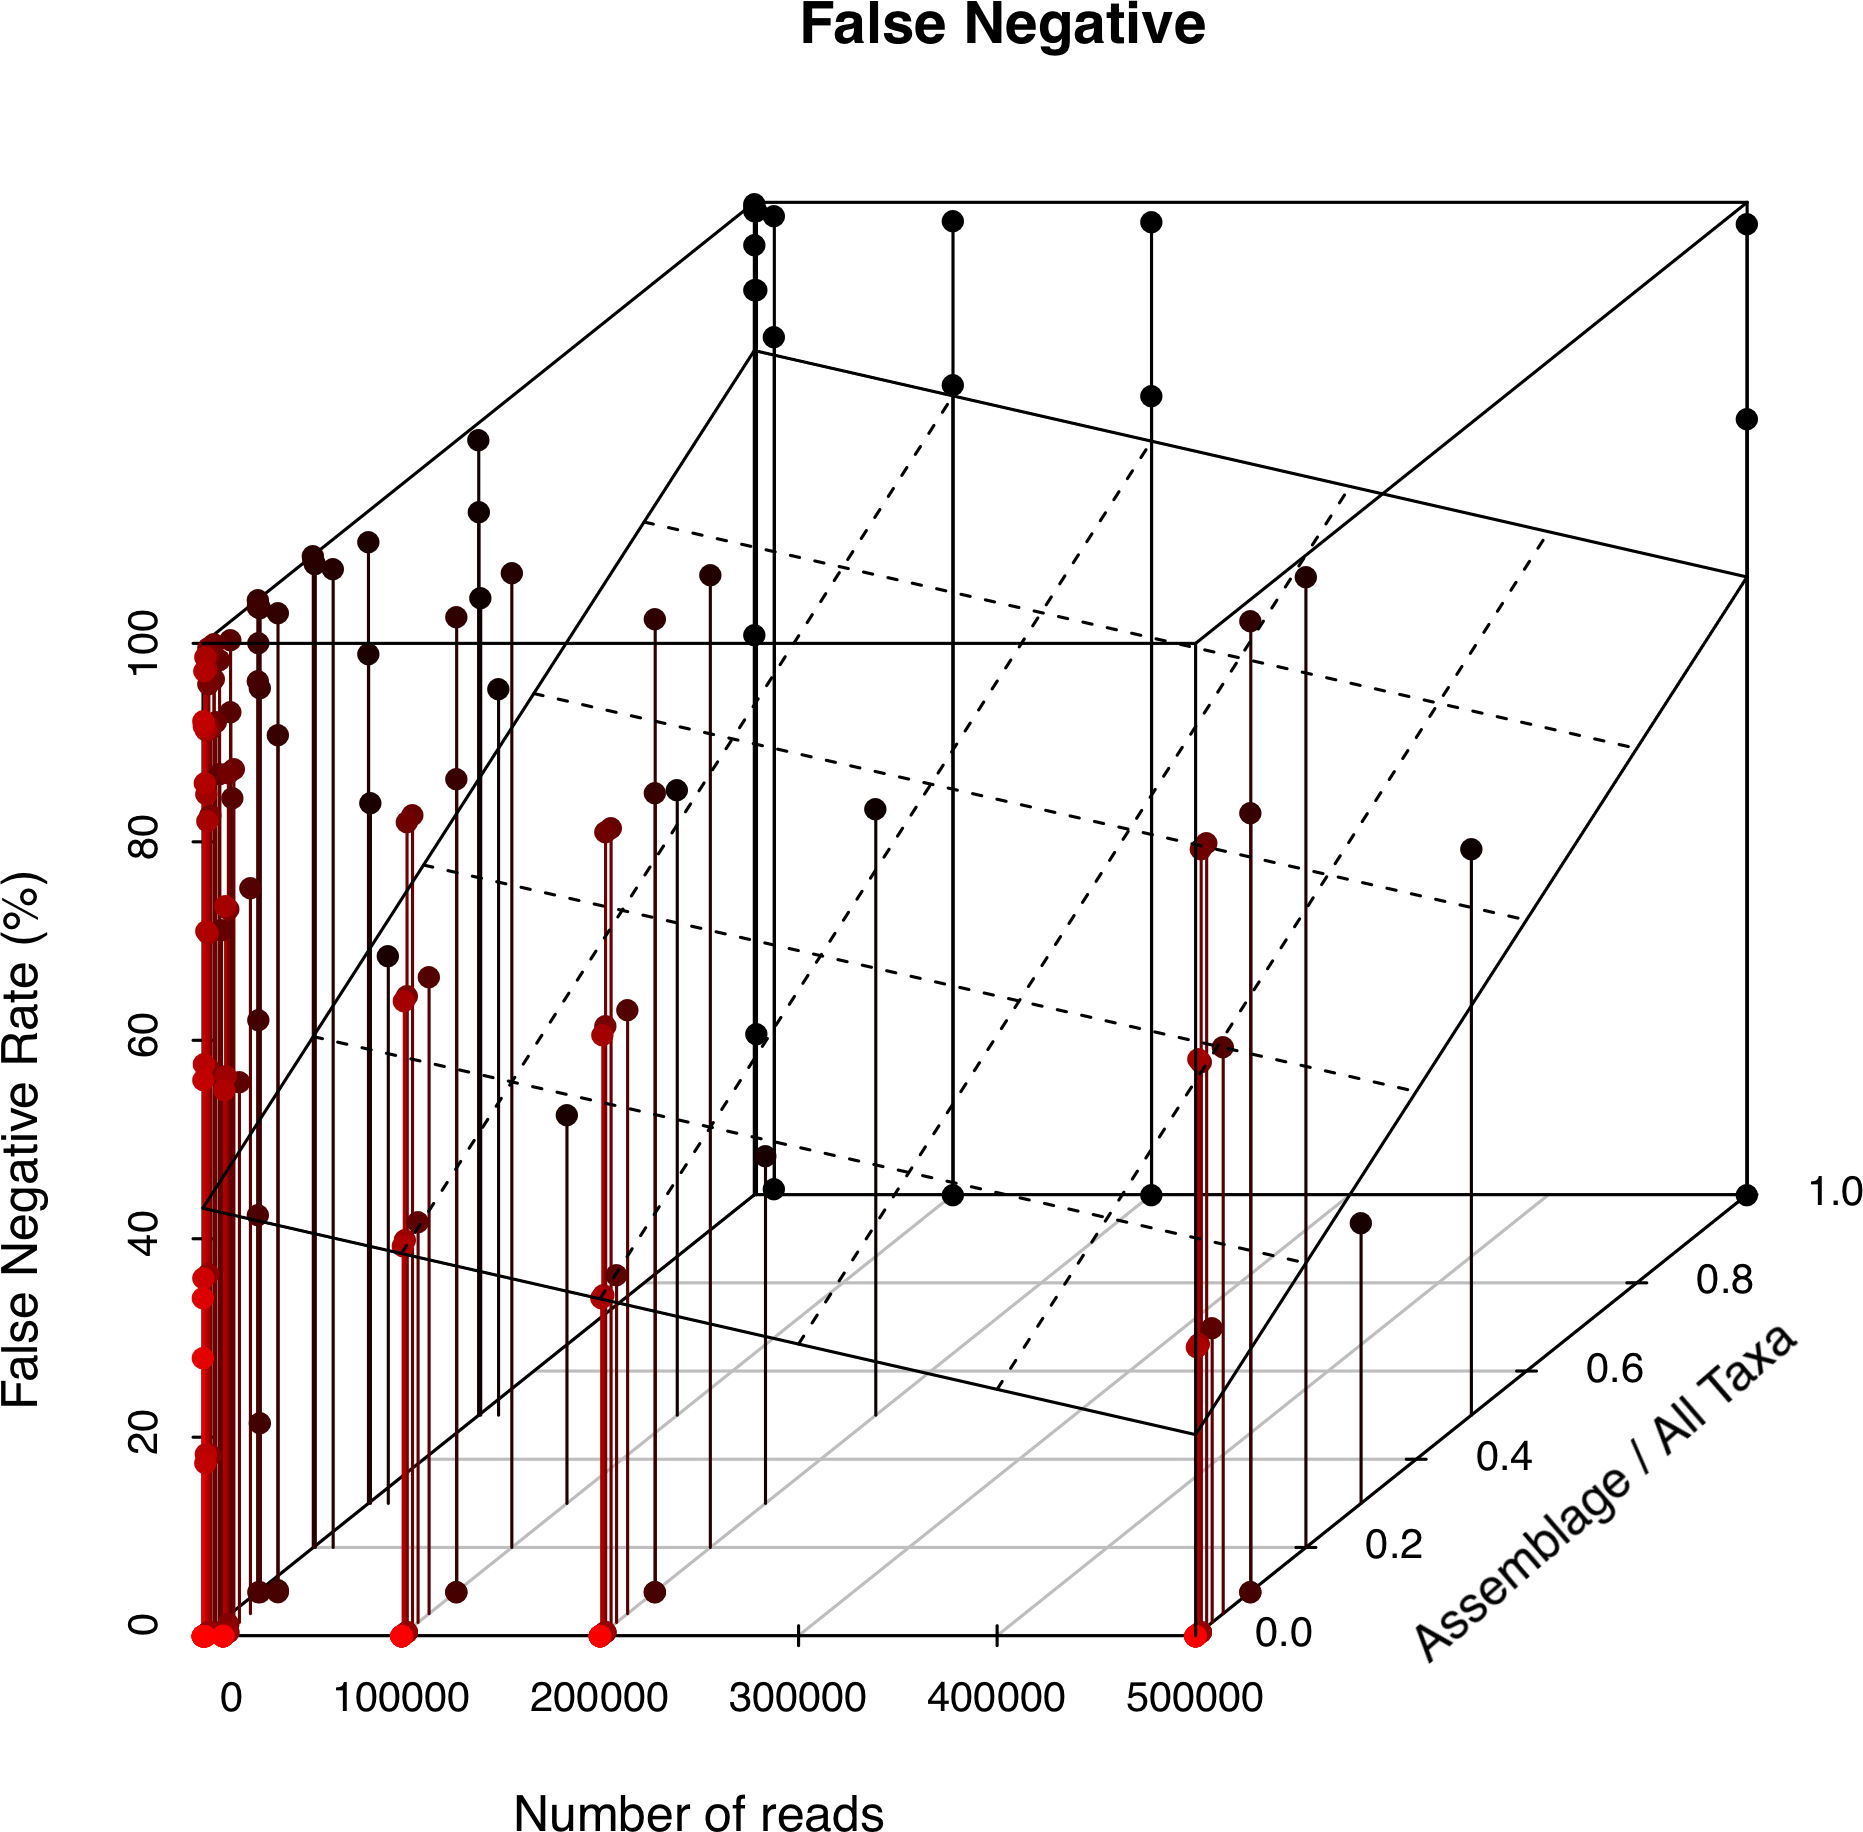
\includegraphics[width=\textwidth]{../polarfront/falsenegative.png}
\caption{TODO false negative}
\label{fig:minspecvalidationfalsenegative}
\end{subfigure}%

&
%\quad %add desired spacing between images, e. g. ~, \quad, \qquad etc. 
%(or a blank line to force the subfigure onto a new line)

\begin{subfigure}[b]{0.5\textwidth}
\centering
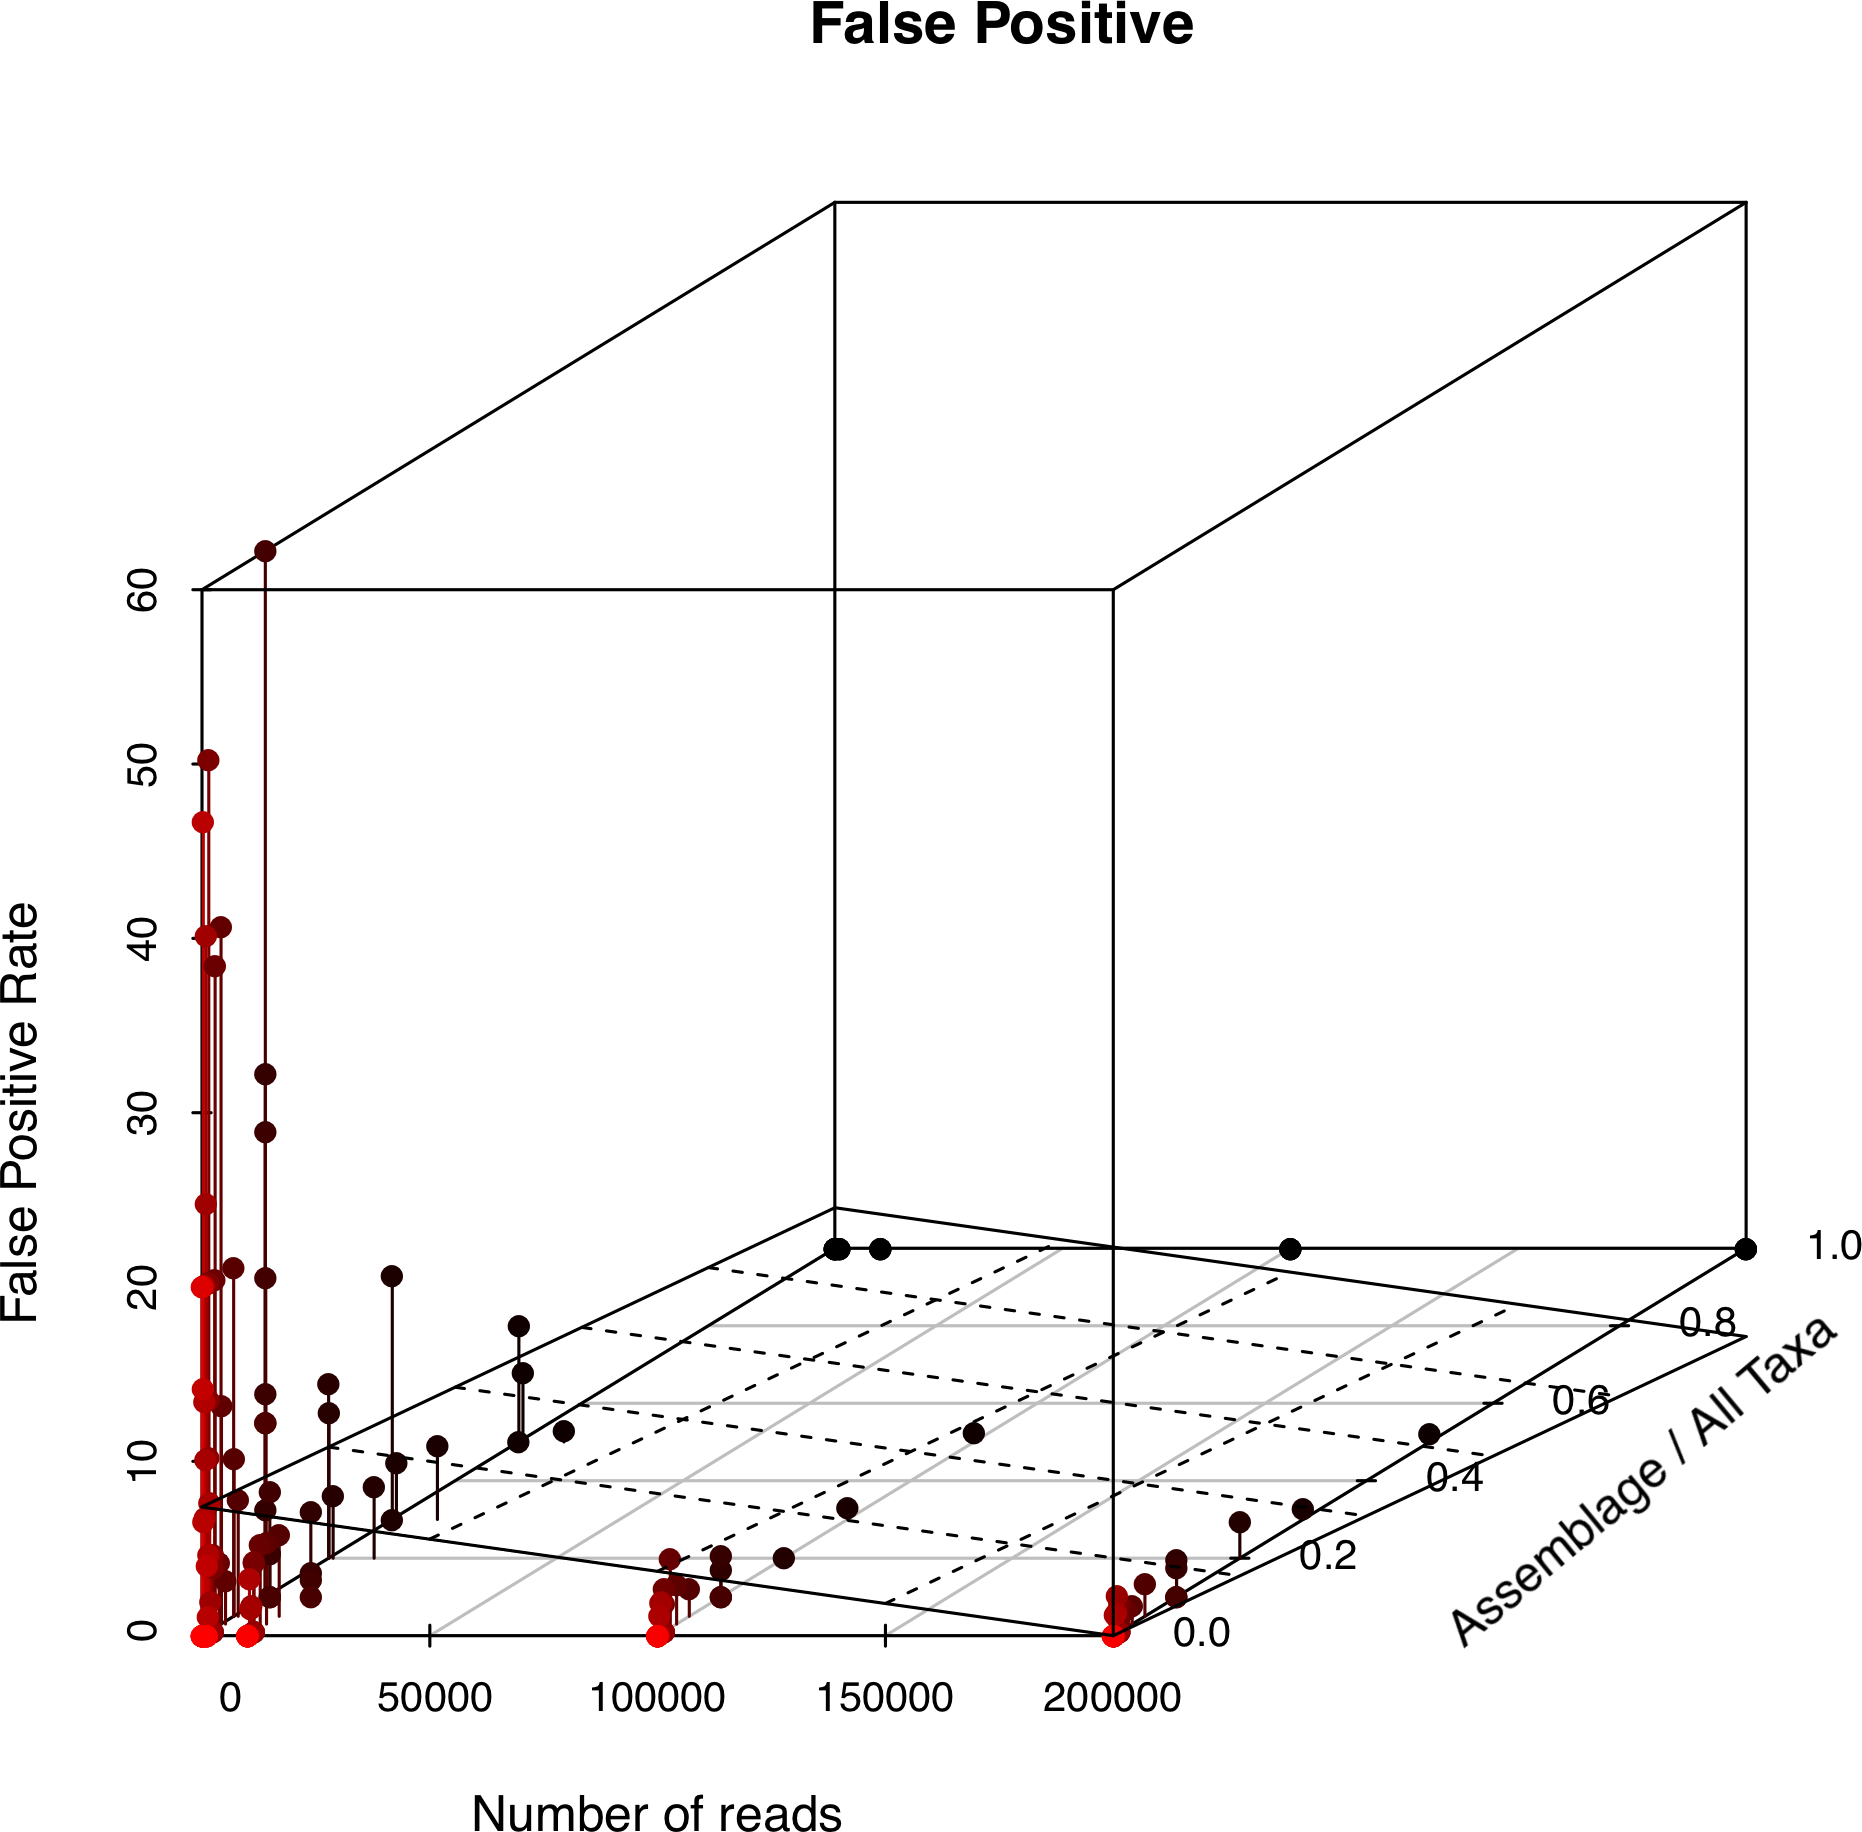
\includegraphics[width=\textwidth]{../polarfront/falsepositive.png}
\caption{TODO false positive}
\label{fig:minspecvalidationfalsepositive}
\end{subfigure}

\\
\bigskip
%\quad %add desired spacing between images, e. g. ~, \quad, \qquad etc. 
%(or a blank line to force the subfigure onto a new line)

\begin{subfigure}[b]{0.5\textwidth}
\centering
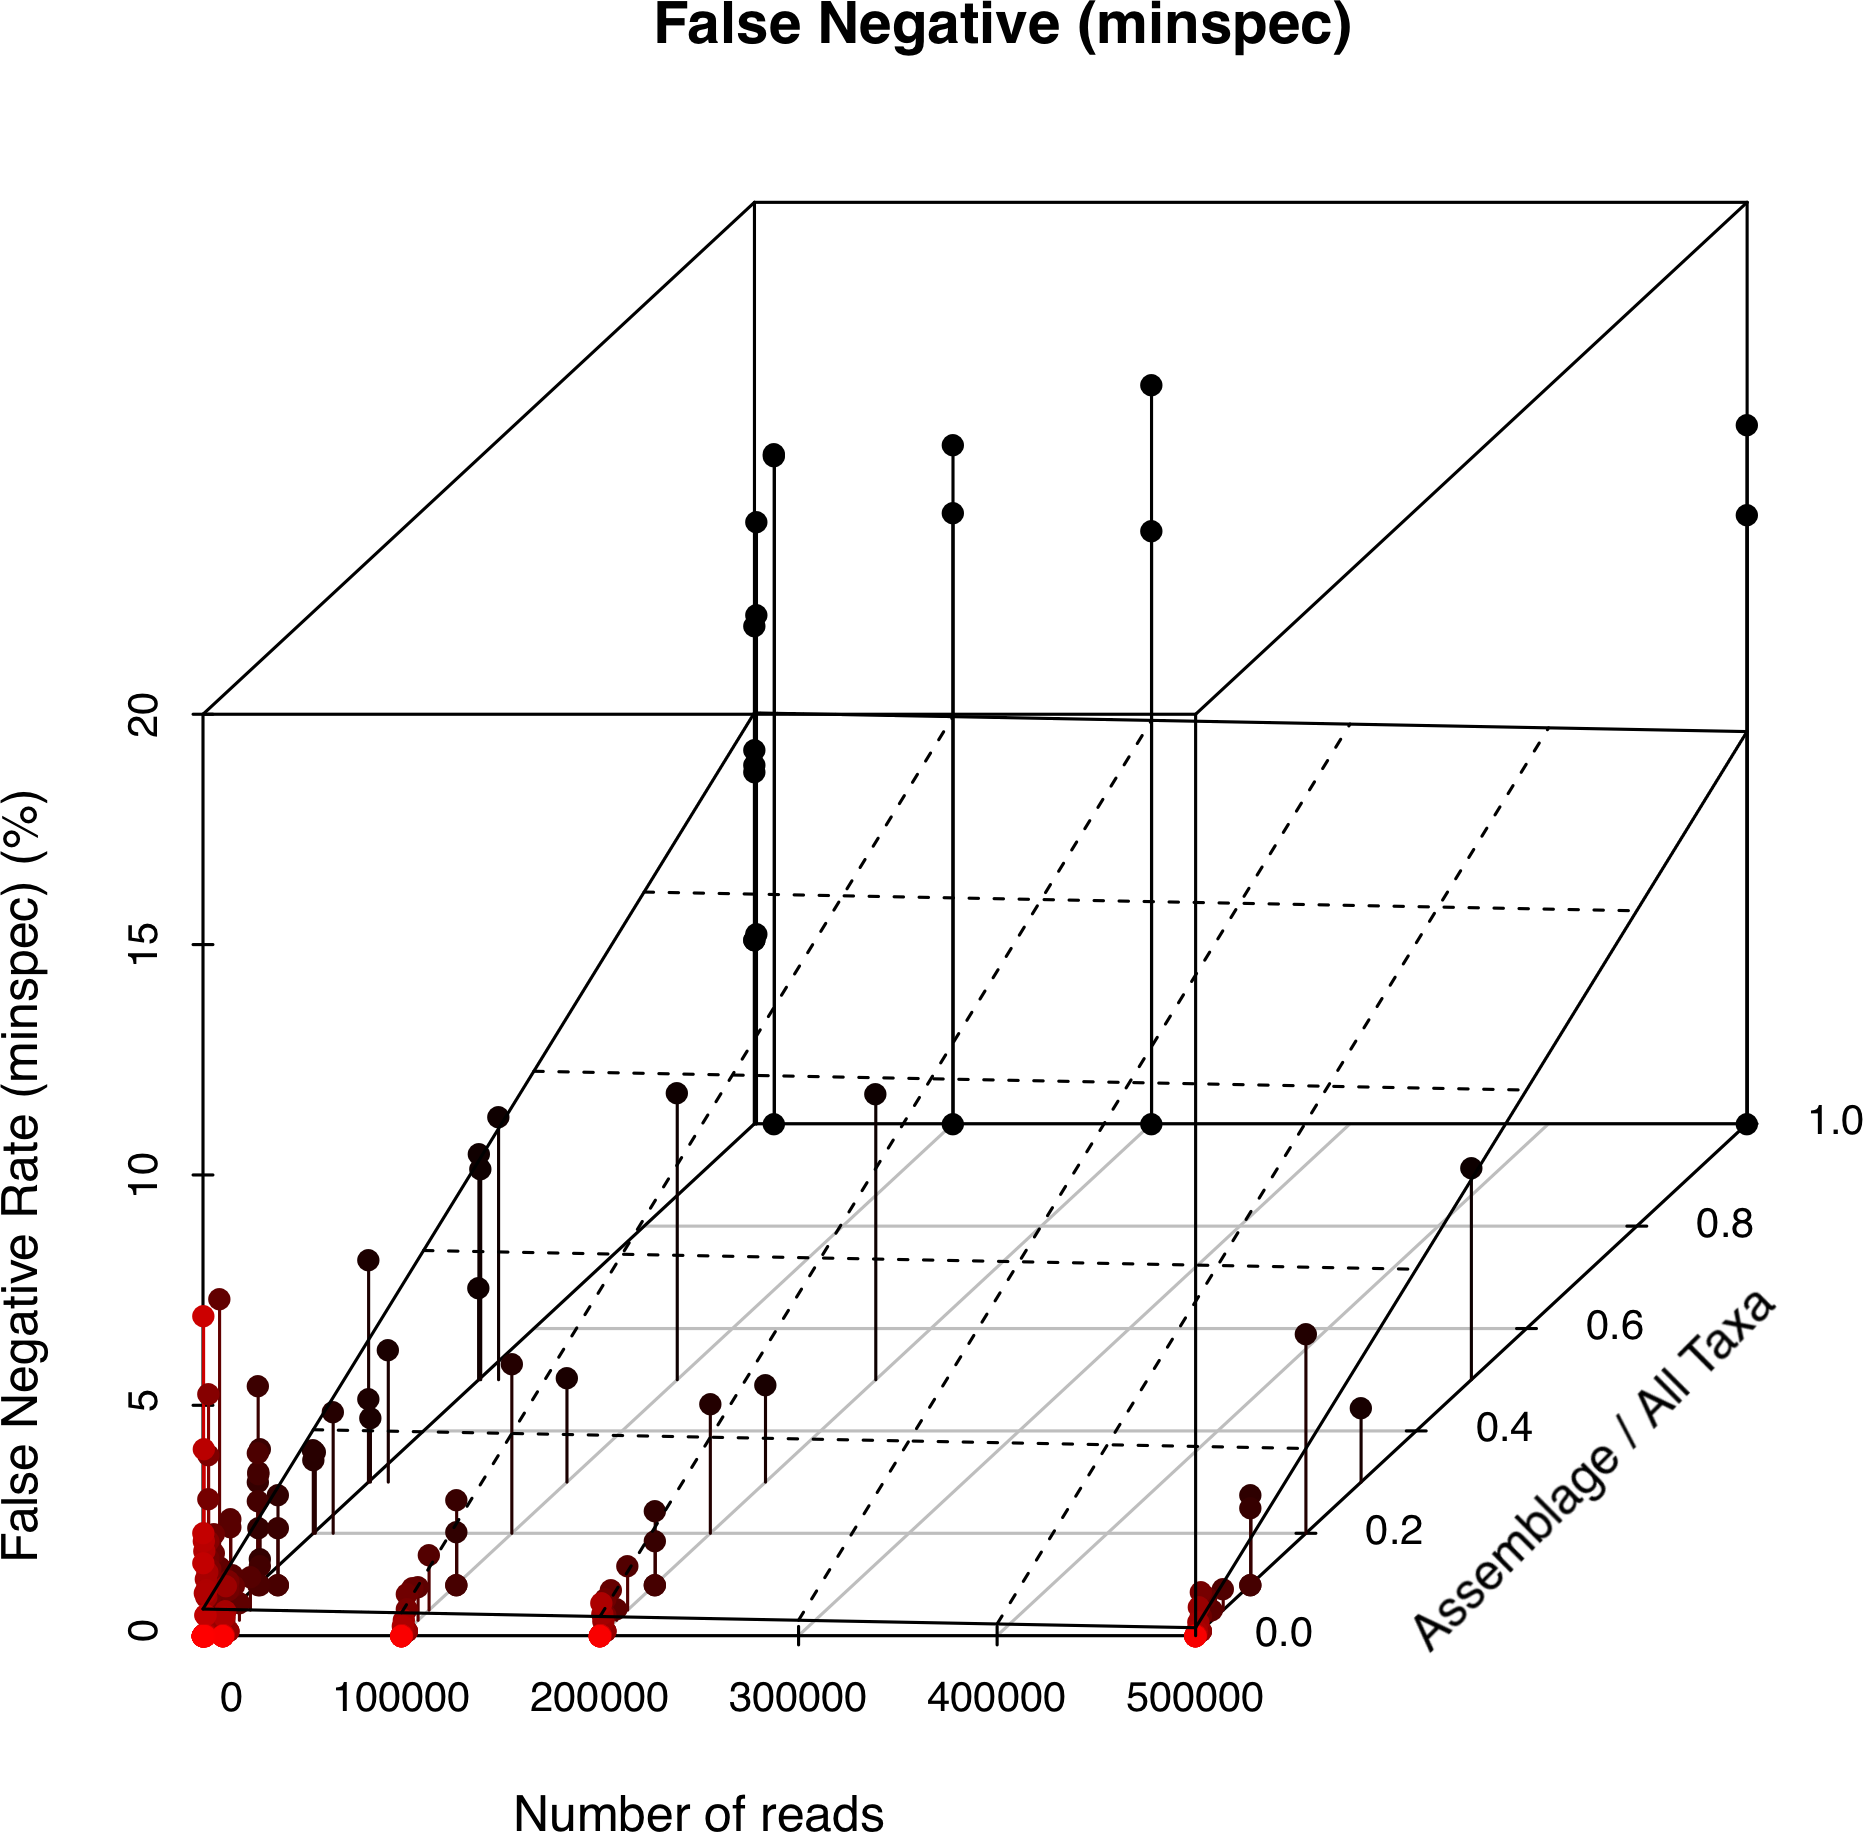
\includegraphics[width=\textwidth]{../polarfront/minspecfalsenegative.png}
\caption{TODO minspec false negative}
\label{fig:minspecvalidationminspecfalsenegative}
\end{subfigure}

&
%\quad %add desired spacing between images, e. g. ~, \quad, \qquad etc. 
%(or a blank line to force the subfigure onto a new line)

\begin{subfigure}[b]{0.5\textwidth}
\centering
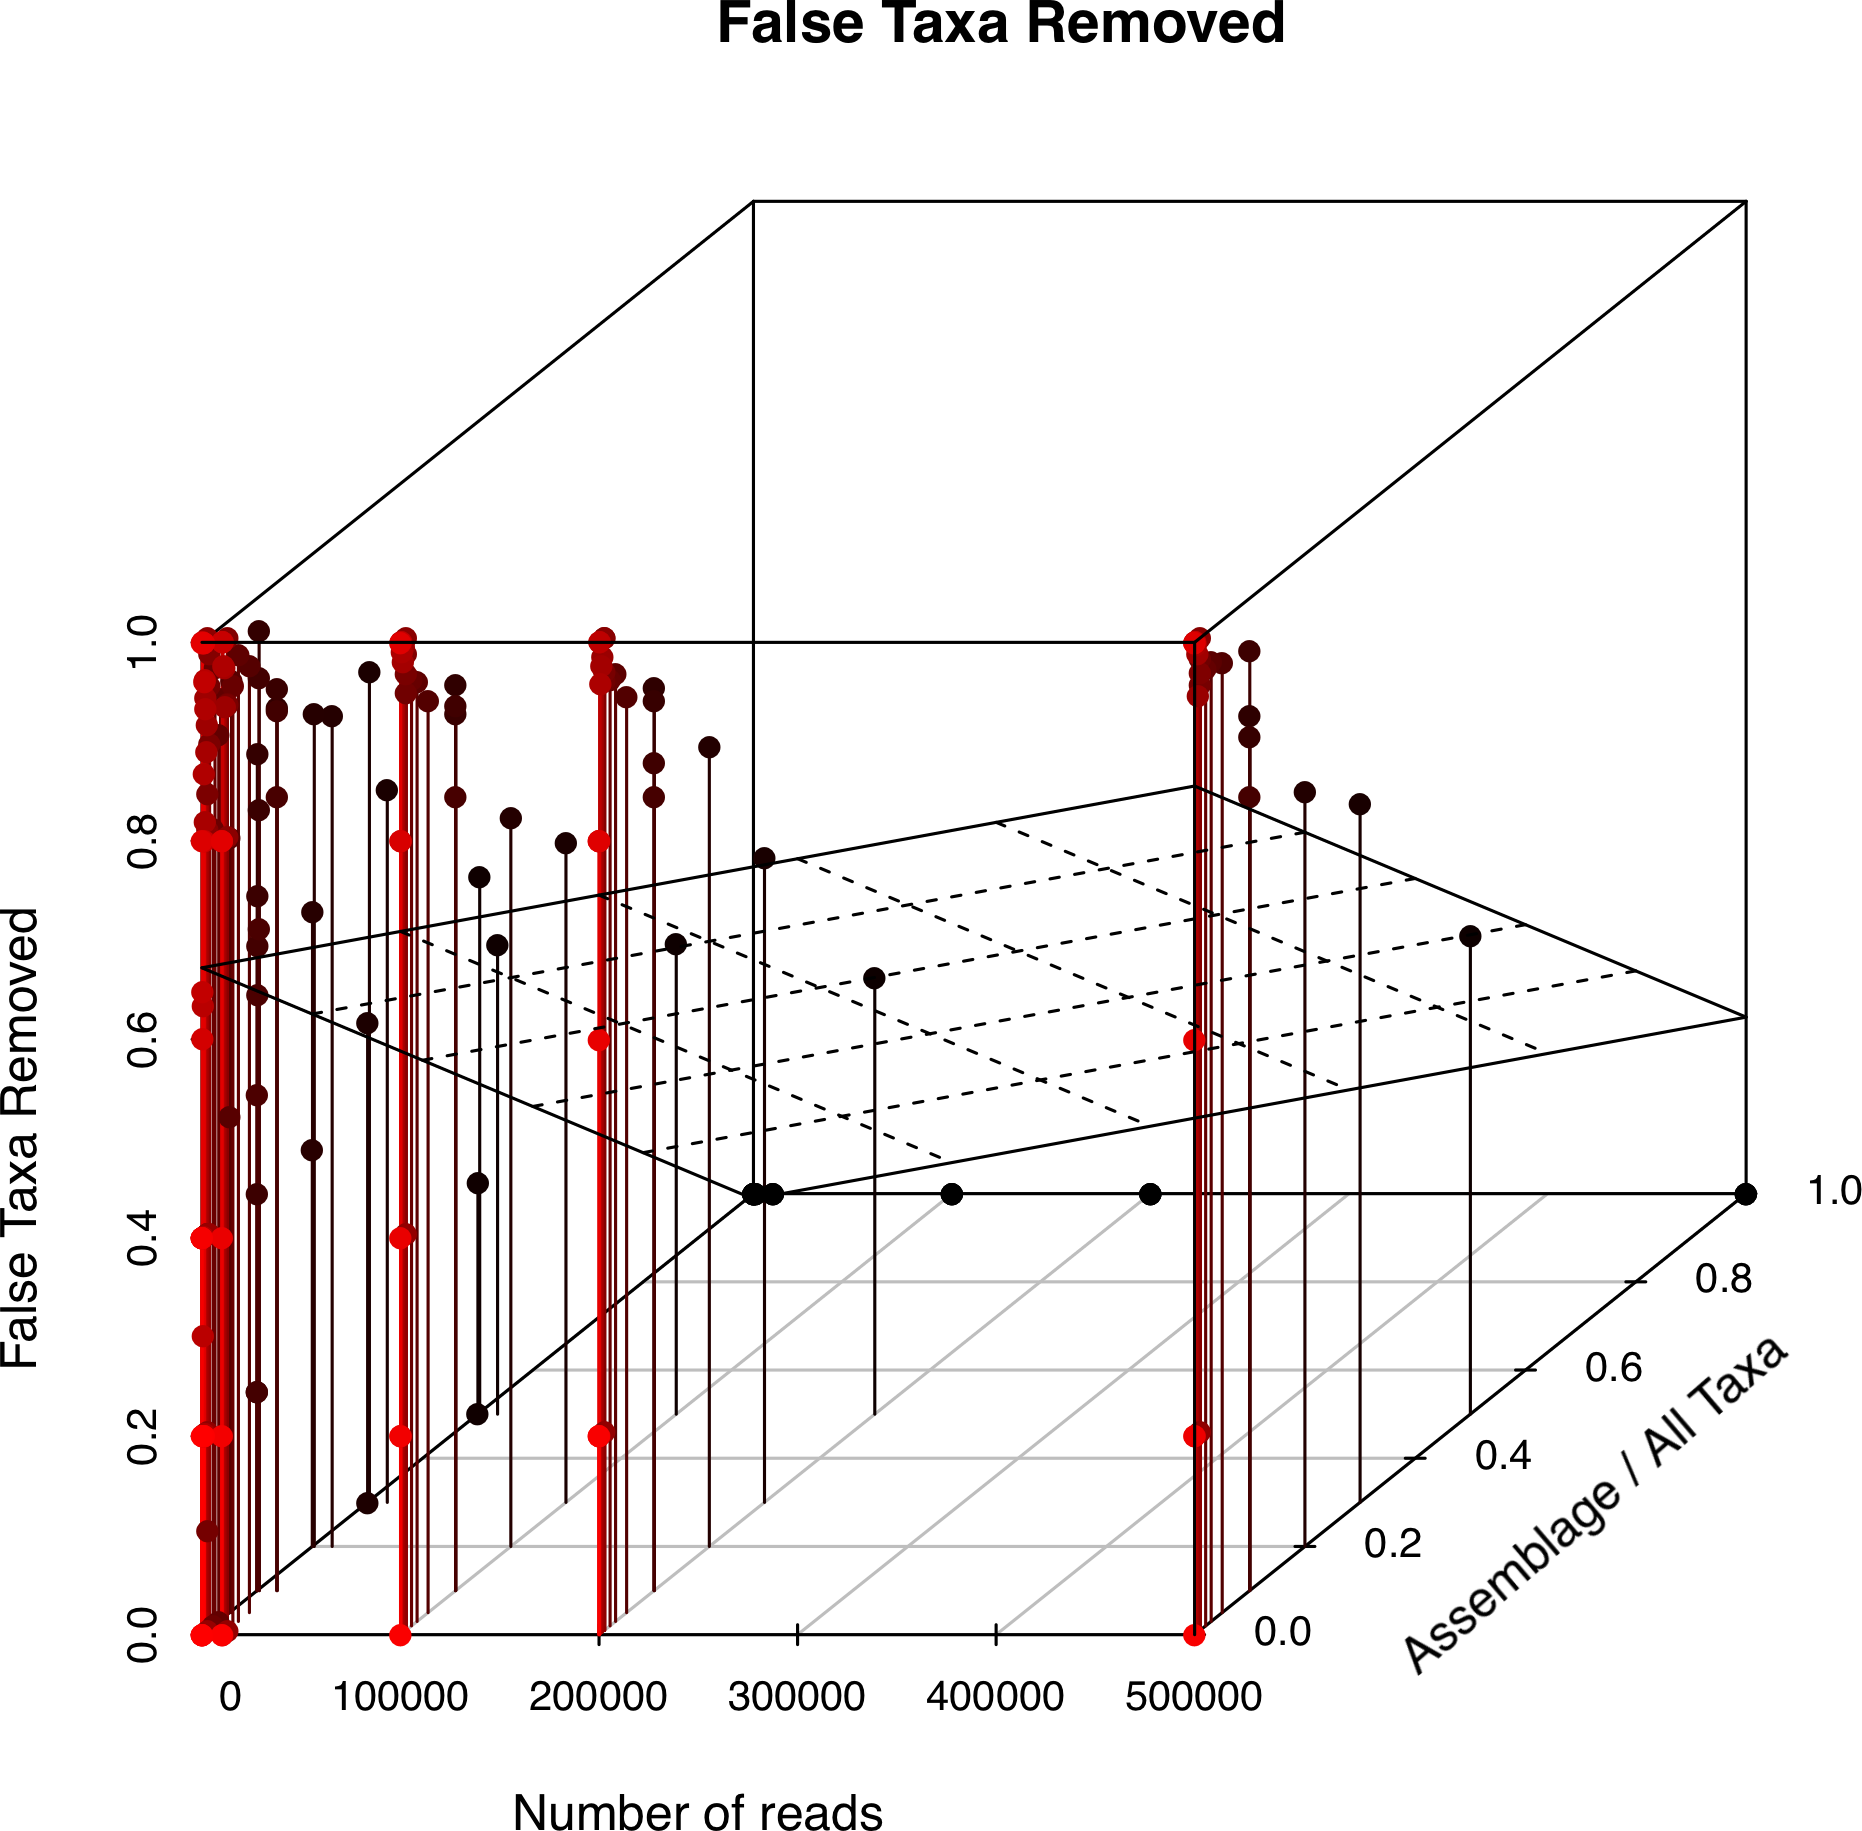
\includegraphics[width=\textwidth]{../polarfront/falsetaxaremoved.png}
\caption{TODO minspec false taxa removed}
\label{fig:minspecvalidationfalsetaxaremoved}
\end{subfigure}
\\

\end{tabular}

\caption{TODO master caption}\label{fig:minspecvalidation}
\end{figure}


The false negative rate, or percentage of taxa in the assemblage which were absent from the \softwarename{blast} results following \softwarename{minspec} processing, was generally high, ranging from \textapprox{} 20\% under ideal conditions (a low assemblage / all taxa ratio, and 500000-read metagenomic sample) to \textapprox{} 90\% in the worst case (a high assemblage / all taxa ratio and a small metagenomic sample) \figref{fig:minspecvalidationfalsenegative}.
The assemblage / all taxa ratio indicates the proportion of a large group of simulated interrelated taxa (``all taxa'') which was chosen to form the simulated assemblage.
A higher ratio means it is more likely on average that any randomly selected taxon is part of the assemblage, and thus that any individual failure to detect a taxon is incorrect.
This problem is mitigated with increasing read count, as this makes it less likely that a given taxon would go undetected.
It is worth noting that the extreme false negative rates, in some cases 100\%, represent extreme simulated scenarios (e.g. an assemblage of 1 taxon drawn from a pool of 100000), and thus are unlikely to reflect real metagenomic studies.

Because the majority of false negatives are attributable to undersampling and failure of taxa to generate \softwarename{blast} hits --- properties the simulated metagenomic experiments share with real ones --- a second metric, the false negative (\softwarename{minspec}) rate, was calculated \figref{fig:minspecvalidationminspecfalsenegative}.
This is the proportion of taxa in the assemblage which generated \softwarename{blast} hits, but were incorrectly removed by \softwarename{minspec}.
This rate thus represents error attributable only to \softwarename{minspec}.
The false negative (\softwarename{minspec}) rate was generally low, ranging from \textapprox{} 0--1\% for low assemblage / all taxa ratios, to \textapprox{} 15--20\% under high ratios.
Surprisingly, increasing read counts only slightly decreased the rate, at both low and high assemblage / all taxa ratios.
This may be because \softwarename{minspec} requires only one read which has identity to a single taxon to ensure that taxon is not removed.

The false positive rate, or percentage of taxa not in the assemblage which were present in the \softwarename{blast} results following \softwarename{minspec} processing, was generally \textapprox{} 0--5\% except for extremely small read sets and low assemblage / all taxa ratios, where it reached as high as 60\%.
As with the false negative rate, false positive results cannot be attributed soley to \softwarename{minspec}; they are the very problem \softwarename{minspec} was designed to address.
These results reinforce the value of larger read sets, and show that once a modest metagenome size is reached (\textapprox{} 100000 reads) very few false positives can be expected.



TODO UP TO HERE

\subsection{Functional analysis of metagenomic data}

TODO working on this section

\ac{ANOSIM} analysis of the samples' \ac{KEGG} ortholog group and module profiles revealed that the zones had significantly different functional potential (ortholog group: R = 0.642, p < 0.001; module: R = 0.871, p < 0.001). 
\ac{SIMPER} was performed on the profiles in order to identify the specific functional differences between the zones. 
The highest-contributing modules are given in \tabreft{tab:modulessimper}, and a complete list in the supplementary material \suppfile{PF-modules-SIMPER.csv}.
The highest-contributing ortholog groups are given in \tabreft{tab:orthologsimper}, and a complete list in the supplementary material \suppfile{PF-ortholog-groups-SIMPER.csv}.
No single ortholog group or module contributed more than 2.2\% of the variance, indicating a complex and diverse pattern of functional differences. 
There was a strong trend for ortholog groups and modules with higher contributions to variance to be overrepresented in the \ac{NZ} in the 3.0 \micron{} fraction but the \ac{SZ} in the smaller fractions, indicating that the functional diversity of each zone was strongly segregated by size fraction.

\begin{sidewaystable}
\sffamily
\begin{center}
\caption[Contributions of KEGG modules to variance between the North and South zones]{\sffamily{}The thirty \ac{KEGG} modules with the highest contributions to the difference between the \ac{NZ} and \ac{SZ}.
Abundances are zonal averages and have been standardised and log-transformed.
}
\label{tab:modulessimper}
\smallskip
\begin{tabularx}{\textwidth}{Xlll}
\toprule
\textbf{\ac{KEGG} module} & \textbf{Abundance} & \textbf{Abundance} & \textbf{Contribution to}\\
& \textbf{South} & \textbf{North} & \textbf{variance (\%)}\\
\midrule
Photosystem II & 0.42 & 0.57 & 2.21\\
Complex I (NADH dehydrogenase), NADH dehydrogenase I/diaphorase subunit of the bidirectional hydrogenase & 0.01 & 0.24 & 1.80\\
Photosystem I & 0.43 & 0.34 & 1.70\\
Pyrimidine deoxyribonucleotide biosynthesis, CDP/CTP \textrightarrow{} dCDP/dCTP,dTDP/dTTP & 0.51 & 0.66 & 1.16\\
Histidine degradation, histidine \textrightarrow{} N-formiminoglutamate \textrightarrow{} glutamate & 0.42 & 0.31 & 1.14\\
Methionine salvage pathway & 0.29 & 0.43 & 1.14\\
sn-Glycerol 3-phosphate transport system & 0.29 & 0.16 & 1.11\\
Complex I (NADH dehydrogenase), NADH dehydrogenase I & 1.08 & 1.05 & 1.06\\
Branched-chain amino acid transport system & 0.79 & 0.83 & 0.96\\
Dipeptide transport system & 0.14 & 0.02 & 0.95\\
Adenine nucleotide biosynthesis, IMP \textrightarrow{} ADP/dADP,ATP/dATP & 0.62 & 0.74 & 0.95\\
Glycine betaine/proline transport system & 0.66 & 0.56 & 0.94\\
Sulfur reduction, sulfate \textrightarrow{} H2S & 0.54 & 0.44 & 0.91\\
Simple sugar transport system & 0.46 & 0.39 & 0.90\\
Peptides/nickel transport system & 0.99 & 0.98 & 0.89\\
Ribosome, eukaryotes & 0.26 & 0.27 & 0.89\\
Multiple sugar transport system & 0.55 & 0.55 & 0.86\\
Type II general secretion system & 0.21 & 0.21 & 0.82\\
Sulfonate/nitrate/taurine transport system & 0.45 & 0.37 & 0.82\\
Guanine nucleotide biosynthesis, IMP \textrightarrow{} GDP/dGDP,GTP/dGTP & 0.72 & 0.82 & 0.81\\
RNA polymerase II, eukaryotes & 0.11 & 0.20 & 0.76\\
Histidine biosynthesis, PRPP \textrightarrow{} histidine & 0.94 & 0.86 & 0.76\\
Putrescine transport system & 0.18 & 0.09 & 0.72\\
Leucine biosynthesis, pyruvate \textrightarrow{} 2-oxoisovalerate \textrightarrow{} leucine & 1.29 & 1.37 & 0.71\\
C5 isoprenoid biosynthesis, non-mevalonate pathway & 0.70 & 0.77 & 0.71\\
Leucine degradation, leucine \textrightarrow{} acetoacetate + acetyl-CoA & 0.64 & 0.59 & 0.71\\
Thiamine transport system & 0.13 & 0.05 & 0.69\\
Spliceosome, 35S U5-snRNP & 0.18 & 0.20 & 0.68\\
Cytochrome b6f complex & 0.14 & 0.12 & 0.67\\
Menaquinone biosynthesis, chorismate \textrightarrow{} menaquinone & 0.25 & 0.27 & 0.66\\
\bottomrule
\end{tabularx}
\end{center}
\end{sidewaystable}

\begin{landscape}
\begin{table}
\sffamily
\begin{center}
\caption[Contributions of KEGG ortholog groups to variance between the North and South zones]{\sffamily{}
The thirty \ac{KEGG} ortholog groups with the highest contribution to the difference between the \ac{NZ} and \ac{SZ}.
Abundances are zonal averages and have been standardised and log-transformed.
As each ortholog group on each size fraction was encoded as a separate variable in the \ac{SIMPER} analysis, the size fraction is given after each ortholog group name.
}
\label{tab:orthologsimper}
\smallskip
\begin{tabularx}{\linewidth}{Xlll}
\toprule
\textbf{KEGG ortholog group} & \textbf{Abundance} & \textbf{Abundance} & \textbf{Contribution to}\\
& \textbf{South} & \textbf{North} & \textbf{variance (\%)}\\
\midrule
Hypothetical protein 3.0 \micron & 0.11 & 0.24 & 0.26\\
Hypothetical protein 0.8 \micron & 0.68 & 0.57 & 0.24\\
Ribonucleoside-diphosphate reductase alpha chain [EC:1.17.4.1] 0.8 \micron & 0.17 & 0.24 & 0.15\\
DNA polymerase III subunit alpha [EC:2.7.7.7] 0.8 \micron & 0.25 & 0.19 & 0.14\\
Hypothetical protein 0.1 \micron & 0.26 & 0.24 & 0.12\\
Proline dehydrogenase / delta 1-pyrroline-5-carboxylate 0.8 \micron & 0.10 & 0.04 & 0.12\\
Aminomethyltransferase [EC:2.1.2.10] 0.8 \micron & 0.25 & 0.19 & 0.12\\
Ribonucleoside-diphosphate reductase alpha chain [EC:1.17.4.1] 3.0 \micron & 0.02 & 0.08 & 0.12\\
Sarcosine oxidase, subunit alpha [EC:1.5.3.1] 0.8 \micron & 0.22 & 0.17 & 0.12\\
Integrator complex subunit 6 3.0 \micron & 0.07 & 0.05 & 0.11\\
Multicomponent Na$^{+}$:H$^{+}$ antiporter subunit D 0.8 \micron & 0.11 & 0.05 & 0.11\\
Glutamine synthetase [EC:6.3.1.2] 0.8 \micron & 0.24 & 0.19 & 0.11\\
Pyruvate dehydrogenase E1 component [EC:1.2.4.1] 0.8 \micron & 0.15 & 0.10 & 0.11\\
Cobaltochelatase CobN [EC:6.6.1.2] 0.8 \micron & 0.11 & 0.06 & 0.11\\
Formate dehydrogenase, alpha subunit [EC:1.2.1.2] 0.8 \micron & 0.15 & 0.10 & 0.11\\
DNA-directed RNA polymerase subunit beta [EC:2.7.7.6] 3.0 \micron & 0.03 & 0.08 & 0.11\\
Glutamate synthase (NADPH/NADH) large chain [EC:1.4.1.13 1.4.1.14] 0.8 \micron & 0.25 & 0.22 & 0.11\\
Dimethylglycine dehydrogenase [EC:1.5.99.2] 0.8 \micron & 0.17 & 0.14 & 0.11\\
Flagellin 0.8 \micron & 0.06 & 0.10 & 0.10\\
DNA-directed RNA polymerase subunit beta [EC:2.7.7.6] 3.0 \micron{}\footnote{Due to an error in the \ac{KEGG} database, this module is encoded twice.} & 0.03 & 0.08 & 0.10\\
Photosystem II PsbA protein 0.8 \micron & 0.01 & 0.06 & 0.09\\
Aldehyde dehydrogenase (NAD+) [EC:1.2.1.3] 0.8 \micron & 0.17 & 0.13 & 0.09\\
Glutamate synthase (NADPH/NADH) large chain [EC:1.4.1.13 1.4.1.14] 3.0 \micron & 0.02 & 0.07 & 0.09\\
Thymidylate synthase (FAD) [EC:2.1.1.148] 0.8 \micron & 0.02 & 0.06 & 0.09\\
Topoisomerase IV subunit A [EC:5.99.1.-] 0.8 \micron & 0.11 & 0.07 & 0.09\\
DNA mismatch repair protein MutS 0.8 \micron & 0.13 & 0.08 & 0.09\\
Glutamate dehydrogenase [EC:1.4.1.2] 0.8 \micron & 0.07 & 0.03 & 0.09\\
DNA polymerase I [EC:2.7.7.7] 0.1 \micron & 0.12 & 0.11 & 0.09\\
GTP-binding protein 0.8 \micron & 0.26 & 0.21 & 0.09\\
GTP-binding protein 3.0 \micron & 0.03 & 0.07 & 0.09\\
\bottomrule
\end{tabularx}
\end{center}
\end{table}
\end{landscape}


\section{Discussion}

\section{Conclusions}

